\documentclass[11pt,a4paper]{article}
\usepackage[T1]{fontenc}
\usepackage{textcomp}
\usepackage{lmodern,microtype,amsmath,amssymb,amsthm,mathtools}
\usepackage[a4paper,top=24mm,bottom=25mm,left=24mm,right=24mm]{geometry}
\usepackage{booktabs,array,longtable,enumitem,xcolor,tikz,listings,fancyhdr}
\usepackage[colorlinks=true,linkcolor=navy,citecolor=navy,urlcolor=teal]{hyperref}
\definecolor{navy}{RGB}{21,43,72}
\definecolor{teal}{RGB}{0,111,117}
\definecolor{muted}{RGB}{86,99,111}
\definecolor{light}{RGB}{244,247,249}
\definecolor{rust}{RGB}{175,64,40}
\usetikzlibrary{arrows.meta,calc}
\pagestyle{fancy}\fancyhf{}
\fancyhead[L]{\small\color{muted}Composed mathematical certificates}
\fancyhead[R]{\small\color{muted}Keio and Shaitetsu}
\fancyfoot[C]{\small\thepage}
\setlength{\headheight}{14pt}
\setlength{\parskip}{4pt}
\setlength{\parindent}{0pt}
\setlength{\emergencystretch}{2em}
\renewcommand{\arraystretch}{1.16}
\setcounter{tocdepth}{2}
\newtheorem{theorem}{Theorem}[section]
\newtheorem{lemma}[theorem]{Lemma}
\newtheorem{corollary}[theorem]{Corollary}
\newtheorem{proposition}[theorem]{Proposition}
\theoremstyle{definition}
\newtheorem{definition}[theorem]{Definition}
\newtheorem{example}[theorem]{Example}
\theoremstyle{remark}\newtheorem{remark}[theorem]{Remark}
\DeclareMathOperator{\tr}{tr}
\DeclareMathOperator{\Cov}{Cov}
\DeclareMathOperator{\Var}{Var}
\lstset{language=Python,basicstyle=\ttfamily\scriptsize,
  backgroundcolor=\color{light},frame=single,rulecolor=\color{muted!30},
  breaklines=true,columns=fullflexible,keepspaces=true,
  showstringspaces=false,upquote=true,tabsize=4}
\hypersetup{pdftitle={Composed Certificates: Weighted Wheels, Sharp Stability, and Arithmetic Tail Laws},
 pdfauthor={Keio and Shaitetsu},pdfsubject={Research manuscript with complete proofs and exact verification}}

\begin{document}
\begin{titlepage}
\color{navy}
{\small\sffamily CONTINUED RESEARCH MANUSCRIPT\hfill 19 NOVEMBER 2026}\par
\vspace{17mm}
{\LARGE\bfseries Composed Certificates}\par
\vspace{5mm}
{\Large Weighted Wheels, Sharp Stability,\\[3pt]
and Arithmetic Tail Laws}\par
\vspace{6mm}
{\large Keio and Shaitetsu}\par
\vspace{10mm}
\color{black}
\textbf{Main result.} For every wheel graph $W_n=K_1+C_n$, $n\ge3$,
every positive assignment of edge activities, and every $0<q<1$, the
random-cluster measure has strictly negative pairwise edge correlation.
The proof deforms a forest transfer matrix, proves two new inequalities
for every word in its matrix semigroup, and converts them into explicit
Rayleigh certificates for all three types of edge pairs.

\medskip
\textbf{Continuation.} The theorem extends to arbitrary finite nested
two-terminal compositions of wheels and cycles, including the cone over
every connected cactus graph. Further coupled invariants give
coefficientwise certificates and explicit correlation bounds. A
three-terminal analysis isolates the exact additional inequality needed
for the next extension, and proves that positivity of boundary
coordinates alone is insufficient.

\medskip
\textbf{Three additional developments.} We determine the exact region in
which a parity transversal is optimal, including uniqueness on the critical
line and its optimal H\"older stability exponent. For the one-omission
Erd\H{o}s--Graham construction, we prove that multiplicity thresholds have
density $\exp[-\Theta(r^2\log r)]$, strengthening the previous exponential
upper bound. For conditioned prime phases, we identify a fractional
harmonic spectrum, prove concentration for growing harmonics below
$\sqrt\lambda$, and obtain a nondegenerate Gaussian-phase limit at that
critical scale.

\medskip
The Diophantine part also gives a self-contained route back to the
fixed-number-of-summands conjecture of Tengely, Ulas and Zygad\l{}o,
already resolved in the attached preceding manuscript. That inherited
conclusion is not counted as an additional discovery.

\vfill
{\color{teal}\rule{\textwidth}{1.2pt}}\par
\small
\textbf{Scope and review.} The wheel theorem covers an entire infinite
graph family with unrestricted positive weights. The general
arbitrary-graph conjecture and full negative association remain outside
the theorem. All results are accompanied by proofs; symbolic identities
and exact finite certificates have been internally checked. This draft
has not been externally refereed, and historical priority is not asserted.
\end{titlepage}
\setcounter{page}{2}

\begingroup
\small\setlength{\parskip}{0pt}
\tableofcontents
\endgroup
\clearpage

\section{The research target and the ten-tool comparison}
\label{sec:overview}

The starting materials are the supplied 15-page manuscript
\emph{Unbounded multiplicities in the Erd\H{o}s--Graham equation}, dated
16 November 2026~\cite{Previous}, and the 190 TeX manuscripts in the VMRC snapshot
\cite{VMRC}. This document is a new companion manuscript: its proofs and
references are included in this single source file, and it can be compiled
without the preceding PDF or any external figure files.

The external target used for the main result is the pairwise
random-cluster conjecture stated as Conjecture~1.8 in
\c{C}i\c{c}eksiz--Ravichandran~\cite{CR2026}. Its arbitrary-graph form
remains open in that source. Bado~\cite{Bado2026} treats uniform wheel
forests, and VMRC~[188] supplies the weighted forest case. Theorem
\ref{thm:wheel} covers the full interval $0<q<1$ on every weighted wheel.
The smallest wheel $W_3=K_4$ is not presented as a previously unknown
case; the claim is a uniform proof for the unbounded wheel family.

The continued edition adds Sections~\ref{sec:wheel-coefficients}--
\ref{sec:three-terminal}. Two-terminal closure itself is the existing
theorem of Wagner~\cite{Wagner2008}; combining it with the wheel result
gives the larger family in Theorem~\ref{thm:wheel-networks}. The
three-terminal formulas describe the remaining obstruction, not a
completed arbitrary-graph proof.

\begin{center}
\begin{tabular}{>{\raggedright\arraybackslash}p{.24\textwidth}>{\raggedright\arraybackslash}p{.38\textwidth}>{\raggedright\arraybackslash}p{.27\textwidth}}
\toprule
Question & Result in this manuscript & Exact scope\\
\midrule
Random-cluster pairwise correlation & Strict Rayleigh inequalities,
Theorems~\ref{thm:wheel} and \ref{thm:wheel-networks}
& Every wheel and nested wheel network, every positive weight, $0<q<1$\\
Parity extremizers & Exact phase boundary and sharp stability,
Theorem~\ref{thm:parity-stability} & All $a,b>1$ for parity optimality;
critical stability on $b=a+1$\\
One-omission multiplicities & Logarithmic tail scale,
Theorem~\ref{thm:omission-tail-scale} & The explicit one-omission count
$H(k)$, not the full count $N(k)$\\
Prime-phase harmonic defects & Fractional spectrum and a critical
random limit, Theorems~\ref{thm:new-fractional}--\ref{thm:new-critical}
& The explicitly defined conditioned probability model\\
\bottomrule
\end{tabular}
\end{center}

\subsection{A ranked map of creative tools}

The ranking below is a qualitative assessment of the distinctiveness and
transfer potential of mechanisms in this corpus. It is not a ranking of
proved problem importance, and it is not an assertion that the mechanisms
were invented for the first time in these sources. A common word such as
``trace'', ``state'', or ``positivity'' is not, by itself, a mathematical
connection. The last column records the actual role in the present work.

\small
\begin{longtable}{@{}>{\raggedright\arraybackslash}p{.06\textwidth}>{\raggedright\arraybackslash}p{.27\textwidth}>{\raggedright\arraybackslash}p{.30\textwidth}>{\raggedright\arraybackslash}p{.27\textwidth}@{}}
\toprule
Rank & Corpus mechanism & Why it is reusable & Role here\\
\midrule\endfirsthead
\toprule Rank & Corpus mechanism & Why it is reusable & Role here\\\midrule\endhead
1 & [085] Semantic decoder trees & Mutual recursive normal forms construct
models where finite-model searches fail. & Reviewed; no decoder identity
is needed in the accepted proofs.\\
2 & [090] Centered integer remainders and tent rigidity & A long binary
representation is encoded by an exact state recurrence. & Direct starting
point for the one-omission equation and arithmetic synchronization.\\
3 & [004] Prime-phase hulls and tilted local densities & Conditioning at a
complex sum can be controlled by Fourier inversion. & Directly extended
to moving harmonic scales and a Gaussian bridge.\\
4 & [141] Harmonic mass and compactness & A family of branches can be
controlled collectively by its total exceptional mass. & Adapted
finite-truncation/tail strategy; no Mills theorem is assumed.\\
5 & [151] Two-state $p$-adic lifting & An auxiliary state makes rank-one
reduction survive repeated digit operations. & Useful model for searching
coupled invariants; its arithmetic theorem is not invoked.\\
6 & [178] Frobenius digits and interpolation & Congruence information
forces exact rigidity in a specified constant-term class. & Reviewed;
no valid transfer to the unrestricted problems was established.\\
7 & [002] Reciprocal traces and Faber coordinates & Global traces encode
invariants while separating them from individual branches. & Reviewed;
the wheel's finite transfer trace is proved separately.\\
8 & [140] Weighted parity packing & A dual packing gives an exact
nonnegative decomposition of objective error. & Directly strengthened to
uniqueness and optimal stability by defect propagation.\\
9 & [126] Collision accounting at two spatial scales & Weighted local
identities control events which might escape to infinity. & Reviewed;
the full strip-symbol problem remains unresolved here.\\
10 & [188] $2\times2$ transfer-semigroup certificates & Finite invariant
inequalities certify arbitrarily long weighted products. & Directly
$q$-deformed to prove the main wheel theorem.\\
\bottomrule
\end{longtable}
\normalsize

Two additional corpus mechanisms become useful after the target is
selected: the rotation-invariant deficits of [149] and the positive-kernel
viewpoint in [147,174]. The Hartman--Watson identity provides the precise
external bridge to Bernstein functions. The paper therefore uses several
interlocking methods, while keeping the unused candidates visible rather
than counting a resemblance as an application.

\subsection{The combinations that carry the proofs}

For the wheel theorem the decisive chain is exact cycle-rank enumeration,
rank-one cuts of a cyclic matrix product, normalized semigroup states,
coupled invariant inequalities, and a sum of nonnegative terms. The
auxiliary invariant is essential: the original forest inequality alone
does not survive the $q$-deformation.

For the corner theorem a dual slack identity feeds a terminating defect
path. Charging its ancestors to the stopping event and balancing this
charge against a geometric tail gives the optimal exponent. For the
arithmetic theorem, CRT compatibility is converted into restrictions on
shared large primes; cyclotomic factorization, a smooth-number estimate,
and prime asymptotics then determine the tail scale. For the analytic
theorems, tilted local limits, split-prime conditioning, Bessel Gaussian
scaling, and cancellation of a common random rotation work together.

\clearpage
\begin{figure}[!ht]
\centering
\begin{minipage}{.45\textwidth}\centering
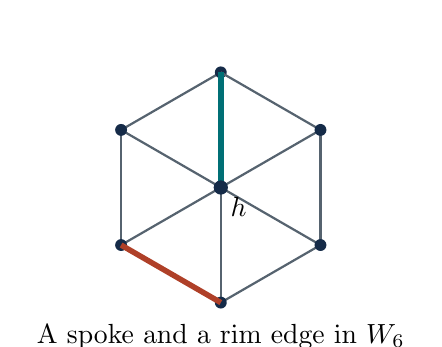
\begin{tikzpicture}[scale=.86]
\coordinate (h) at (0,0);
\foreach \i in {0,...,5}{\coordinate (v\i) at ({90+60*\i}:1.7);}
\foreach \i in {0,...,5}{
 \pgfmathtruncatemacro{\j}{mod(\i+1,6)}
 \draw[muted,line width=.8pt] (v\i)--(v\j);
 \draw[muted,line width=.8pt] (h)--(v\i);
 \fill[navy] (v\i) circle(2.5pt);
}
\draw[teal,line width=2pt] (h)--(v0);
\draw[rust,line width=2pt] (v2)--(v3);
\fill[navy] (h) circle(3pt);
\node[below right] at(h){$h$};
\node at(0,-2.2){A spoke and a rim edge in $W_6$};
\end{tikzpicture}
\end{minipage}\hfill
\begin{minipage}{.5\textwidth}\centering
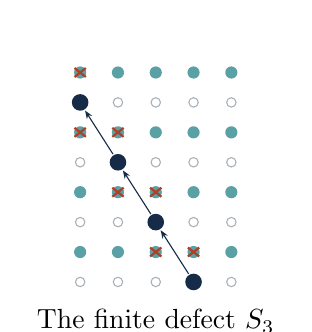
\begin{tikzpicture}[x=.48cm,y=.38cm]
\foreach \i in {0,...,4}{\foreach \j in {0,...,7}{
 \pgfmathtruncatemacro{\odd}{mod(\j,2)}
 \ifnum\odd=1\fill[teal!65] (\i,\j) circle(2.2pt);
 \else\draw[muted!50] (\i,\j) circle(1.7pt);\fi
}}
\foreach \r in {0,...,3}{
 \pgfmathtruncatemacro{\i}{3-\r}
 \pgfmathtruncatemacro{\j}{2*\r}
 \fill[navy] (\i,\j) circle(3pt);
 \pgfmathtruncatemacro{\jj}{2*\r+1}
 \draw[rust,thick] (\i-.15,\jj-.15)--(\i+.15,\jj+.15);
 \draw[rust,thick] (\i-.15,\jj+.15)--(\i+.15,\jj-.15);
 \ifnum\r<3
  \pgfmathtruncatemacro{\ii}{\i-1}
  \draw[rust,thick] (\ii-.15,\jj-.15)--(\ii+.15,\jj+.15);
  \draw[rust,thick] (\ii-.15,\jj+.15)--(\ii+.15,\jj-.15);
  \draw[-{Stealth[length=3pt]},navy] (\i-.13,\j+.27)--(\ii+.13,\j+1.73);
 \fi
}
\node[below] at(2,-.6){The finite defect $S_3$};
\end{tikzpicture}
\end{minipage}
\caption{The proofs keep exact structure. Left: the wheel's cyclic order
reduces all edge pairs to three transfer certificates. Right: added even
vertices (dark) propagate toward column zero; crosses mark deleted odd
vertices. This finite defect witnesses the optimal stability exponent.}
\end{figure}
\section{Negative correlation on weighted wheels throughout \texorpdfstring{$0<q<1$}{0 < q < 1}}
\label{sec:wheel}
Let $W_n=K_1+C_n$ for $n\ge3$, with spoke edges $s_i$ and rim edges $r_i$ (indices cyclic). For a graph $G=(V,E)$ let
\[
 Z_{G,q}(\boldsymbol v)=\sum_{A\subseteq E}q^{k(A)}\prod_{e\in A}v_e,
 \qquad 0<q<1,
\]
where $k(A)$ is the number of components of the spanning subgraph $(V,A)$. Write $\Delta_{ef}Z=Z_eZ_f-ZZ_{ef}$.
\begin{theorem}[Full weighted wheel family]
\label{thm:wheel}
For every $n\ge3$, every $0<q<1$, every positive assignment of edge weights, and distinct edges $e,f$ of $W_n$,
\[
 \Delta_{ef}Z_{W_n,q}>0.
\]
Thus the two edge indicators have strictly negative covariance under the random-cluster measure. The parameter range and all wheel sizes are covered; no assertion for arbitrary graphs follows.
\end{theorem}

\subsection{A deformation of the forest transfer formula}
It is convenient to rescale every edge weight by $q$. Define
\[
 F_q(\boldsymbol w)=q^{-|V|}Z_{W_n,q}(q\boldsymbol w)
 =\sum_{A\subseteq E}q^{|A|+k(A)-|V|}\prod_{e\in A}w_e.
\]
The exponent is the cycle rank. This positive scaling does not change any Rayleigh sign. Put
\[
 P_q(s)=\begin{pmatrix}1&0\\s&1+qs\end{pmatrix},\qquad
 R(t)=\begin{pmatrix}1+t&t\\0&1\end{pmatrix},\qquad c_q=2-q.
\]
Then, writing $t_i=r_i^{-1}$,
\begin{equation}\label{wheel:transfer}
 F_q(\boldsymbol s,\boldsymbol r)=\left(\prod_i r_i\right)H_q(\boldsymbol s,\boldsymbol r^{-1}),
 \qquad H_q=\operatorname{tr}\prod_iP_q(s_i)R(t_i)-c_q.
\end{equation}
To verify this identity, expand $R(t)=I+tU$, with
$U=(1,0)^{\mathsf T}(1,1)$. A nonempty selection of the $tU$ terms specifies the missing rim edges. Each complementary rim path $C$ contributes
\[
 1+\frac{\prod_{i\in C}(1+qs_i)-1}{q}.
\]
Indeed, selecting $\ell\ge1$ spokes in the path produces $\ell-1$ cycles, while selecting none produces none. This is also the scalar factor obtained by splitting the rank-one factors inside the trace, because products of the $P_q(s_i)$ have lower-left entry $[\prod(1+qs_i)-1]/q$ and top-left entry $1$. When no rim edge is missing, the correct factor is
\[
 q+\prod_i(1+qs_i)-1,
\]
which equals the trace of the product of the $P_q(s_i)$ minus $2-q$. Thus all subsets, including the complete rim cycle, have the correct cycle-rank weight.

\subsection{The semigroup invariants}
Let $\mathcal S_q$ consist of products of $P_q(s)$ and $R(t)$ with nonnegative parameters. For
$X=\left(\begin{smallmatrix}a&b\\c&d\end{smallmatrix}\right)\in\mathcal S_q$, set
\[
 D=\det X,\quad A=a+c,\quad B=b+d,\quad A_0=a+qc,\quad B_0=b+qd.
\]
All entries are nonnegative and $D\ge1$. Direct induction gives
\begin{equation}\label{wheel:basic}
 A\ge B\ge D,\qquad A_0\ge D,\qquad B-qA>0,\qquad B_0-qA_0\ge0.
\end{equation}
For completeness, under right multiplication by $P_q(s)$ one has
\[
 (A,B,D)\mapsto(A+sB,(1+qs)B,(1+qs)D),
\]
and under right multiplication by $R(t)$ one has
\[
 (A,B,D)\mapsto((1+t)A,B+tA,(1+t)D).
\]
These preserve $A\ge B\ge D$. The quantities $B-qA$ are unchanged in the first update and increase by $(1-q)tA$ in the second; initially they equal $1-q>0$. For $A_0\ge D$, its first update is $A_0+sB_0$, and $B_0\ge qB\ge qD$; its second update multiplies both sides by $1+t$. Finally, $B_0-qA_0$ is unchanged in the first update and increases by $(1-q)tA_0$ in the second.

We need two less immediate inequalities:
\begin{equation}\label{wheel:UV}
 U(X):=D(a-b)-A_0\ge0,
 \qquad V(X):=Dd(B-qA)-B(B-qD)\ge0.
\end{equation}
Here and below $q$ is fixed in $(0,1)$.

\paragraph{Proof of the first inequality.}
Put $\delta=1-q$ and
\[
 J(X)=\delta b(D-1)+q(A_0-B).
\]
Both $U$ and $J$ vanish at the identity. Right multiplication gives the exact updates
\begin{align*}
 U(XP_q(s))&=(1+qs)U(X)+sJ(X)+q\delta s^2Db,\\
 J(XP_q(s))&=J(X)+\delta bD(2qs+q^2s^2),\\
 U(XR(t))&=(1+t)U(X),\\
 J(XR(t))&=J(X)+\delta t\{U(X)+2Db\}+\delta t^2Da.
\end{align*}
These prove simultaneous nonnegativity of $U$ and $J$.

\paragraph{Proof of the second inequality.}
Normalize $u=A/D$, $v=B/D$. Then $u\ge v\ge1$ and $z=v-qu>0$. The desired inequality is
\[
 \mathcal V=d(v-qu)-v(v-q)\ge0,
 \qquad V(X)=D^2\mathcal V.
\]
Since $Ad-Bc=D$, we have $c=(ud-1)/v$. Right multiplication by $P_q(s)$ changes
\[
 (u,v,d)\mapsto\left(\frac{u+sv}{1+qs},v,(1+qs)d\right),
\]
so $\mathcal V$ is unchanged. For right multiplication by $R(t)$ the update is
\[
 u'=u,\qquad v'=\frac{v+tu}{1+t},\qquad d'=d+t\frac{ud-1}{v}.
\]
The expression $\mathcal V'$ is increasing in $d$, because its coefficient of $d$ is
$(1+tu/v)(v'-qu)>0$. It therefore suffices to substitute the boundary value
$d_*=v(v-q)/z$. Set $x=u-v\ge0$. An exact expansion gives
\begin{equation}\label{wheel:boundary}
 (1+t)^2uvz\,\mathcal V'(d_*)=tC_1+t^2C_2+t^3C_3,
\end{equation}
where
\begin{align*}
 C_1={}&vz(v-1)(v^2+z)
       +x\{v^3(v-1)+z(v^2-z)\}+x^2v^2(v-z),\\
 C_3={}&u(x+z)\{v^2(u-1)+z(v-1)\},\\
 C_2={}&C_1+C_3-uvzx^2.
\end{align*}
We have $0<z\le v\le v^2$, so $C_1,C_3\ge0$. In addition,
\[
 C_3-uvzx^2
 =u\{(v-1)(x+z)(v^2+z)+vx^2(v-z)+v^2xz\}\ge0.
\]
Thus $C_2\ge0$. The invariant is true at the identity and is preserved by both generators, proving the second inequality in \eqref{wheel:UV}. This is a symbolic identity and an induction over arbitrary word length, not an inference from finite numerical checks.

\subsection{Rayleigh certificates for the three edge types}
Since every marked variable occurs affinely in exactly one factor, its Rayleigh difference is independent of the two marked variables. Set those variables to zero, leaving two cyclic segments $X,Y\in\mathcal S_q$.

We use the following elementary identity. For arbitrary two-by-two matrices
$X'=\left(\begin{smallmatrix}\alpha&\beta\\\gamma&\eta\end{smallmatrix}\right)$ and
$Y'=\left(\begin{smallmatrix}\mu&\nu\\\xi&\tau\end{smallmatrix}\right)$, the Rayleigh difference for two insertions of $I+t\operatorname{diag}(1,0)$ in $\operatorname{tr}(\cdot)-c_q$ is
\begin{equation}\label{wheel:rankone}
 D_XD_Y-\alpha\eta D_Y-\mu\tau D_X+c_q\alpha\mu.
\end{equation}
If $\alpha\ge D_X$, $\mu\ge D_Y$, $\beta,\nu\ge0$, and $\gamma,\xi\le0$, then
$\alpha\eta=D_X+\beta\gamma\le D_X$ and similarly for $Y'$. Consequently \eqref{wheel:rankone} is at least
$(c_q-1)D_XD_Y=(1-q)D_XD_Y>0$.

\paragraph{Two rim variables.}
The involution $S=\left(\begin{smallmatrix}1&1\\0&-1\end{smallmatrix}\right)$ conjugates $U=R'(t)$ to $\operatorname{diag}(1,0)$. For $X'=SXS$ its top-left entry is $A$, its top-right entry is $A-B$, and its bottom-left entry is $-c$. The required inequalities follow from \eqref{wheel:basic}. Hence $\Delta_{t_i t_j}H_q>0$.

\paragraph{Two spoke variables.}
The derivative $E_q=P_q'(s)=\left(\begin{smallmatrix}0&0\\1&q\end{smallmatrix}\right)$ is conjugate to $q\operatorname{diag}(1,0)$ by the matrix with columns $(0,1)^{\mathsf T}$ and $(-q,1)^{\mathsf T}$. In these coordinates the top-left, top-right, and bottom-left entries of $X'$ are
\[
 B_0/q,\qquad (B_0-qA_0)/q,\qquad -b/q.
\]
Since $B_0\ge qB\ge qD$, the same certificate applies, with an additional positive factor $q^2$. Hence $\Delta_{s_i s_j}H_q>0$.

\paragraph{One variable of each type.}
Write
$X=\left(\begin{smallmatrix}a&b\\c&d\end{smallmatrix}\right)$ and
$Y=\left(\begin{smallmatrix}e&f\\g&h\end{smallmatrix}\right)$.
Set $A_0=a+qc$, $y=f+h$, $z_Y=y-q(e+g)$ and
$\alpha=A_0/D_X$, $\beta=y/D_Y$. Expansion of
$\operatorname{tr}((I+sE_q)X(I+tU)Y)-c_q$ yields
\[
 K:=-\Delta_{st}H_q
 =A_0(a-b)D_Y+D_Xh z_Y-c_q A_0y.
\]
The exact certificate is
\begin{equation}\label{wheel:mixed}
 \boxed{\frac{K}{D_XD_Y}
 = (\alpha-\beta)^2+q\beta(\alpha-1)
   +\frac{\alpha U(X)}{D_X}+\frac{V(Y)}{D_Y^2}\ge0.}
\end{equation}
All terms are nonnegative by \eqref{wheel:basic} and \eqref{wheel:UV}.
This is strict for a positive wheel. If the marked rim factor does not immediately follow the marked spoke factor, the first segment starts with $R(t)P_q(s)$, for which
$A_0-D=(1-q)st>0$; subsequent right multiplications preserve this strict inequality. Thus $\alpha>1$. In the adjacent case, $X=I$ and $Y$ contains the remaining complete $P_qR$ pairs. Starting with one positive $P_q(s)$ gives $u>v=1$; then a positive $R(t)$ makes the right side of \eqref{wheel:boundary} strictly positive. Thus $V(Y)>0$, and subsequent generators preserve strictness.

\paragraph{Returning to edge weights.}
Let $B_r=\prod_i r_i$. The monomial prefactor in \eqref{wheel:transfer} has no mixed logarithmic derivative. Because $dt_i/dr_i=-r_i^{-2}$, we obtain
\begin{align*}
 \Delta_{s_i s_j}F_q&=B_r^2\Delta_{s_i s_j}H_q,\\
 \Delta_{r_i r_j}F_q&=B_r^2(r_i r_j)^{-2}\Delta_{t_i t_j}H_q,\\
 \Delta_{s_i r_j}F_q&=-B_r^2r_j^{-2}\Delta_{s_i t_j}H_q.
\end{align*}
The three strict signs above prove the theorem. At $q=1$, the random-cluster measure is independent and every Rayleigh difference is zero. At $q=0$ the cycle-rank polynomial reduces to the forest polynomial, consistent with the earlier forest result.

\subsection{Conditioning, minors, and concentration}

\begin{corollary}\label{cor:wheel-conditioning}
Every minor of a wheel satisfies the non-strict pairwise Rayleigh
inequality for $0<q<1$. On a wheel, the same pairwise inequality holds
after any fixed collection of other edge indicators has been prescribed.
Consequently, if $X_e$ are the original edge indicators and
$p_e=\mathbb P(X_e=1)$, then for any edge set $T$,
\[
 \mathbb P(X_e=1\text{ for all }e\in T)\le\prod_{e\in T}p_e,
 \qquad
 \mathbb P(X_e=0\text{ for all }e\in T)\le\prod_{e\in T}(1-p_e).
\]
For nonnegative real numbers $c_e$ and every $\theta\in\mathbb R$,
\begin{equation}\label{wheel:mgf}
 \mathbb E\exp\left(\theta\sum_e c_eX_e\right)
 \le\prod_e\left(1-p_e+p_e e^{\theta c_e}\right).
\end{equation}
\end{corollary}

\begin{proof}
For a multiaffine polynomial $Z$, fixing an edge absent sets its
variable to zero; fixing it present replaces $Z$ by its partial
derivative, up to a constant factor. The Rayleigh inequalities are
preserved by the first operation by continuity. For the second, write
$Z=A+z_gB$ and take the coefficient of $z_g^2$ in a Rayleigh difference
for two other edges: it equals the Rayleigh difference of $B$ and is
nonnegative, since the full difference is nonnegative for all
$z_g>0$. Repeating these operations proves the conditional assertion.
Deletion and contraction give precisely these polynomials up to positive
constant factors; loops contribute independent factors.

Conditional pairwise negative correlation implies that prescribing
one more edge present can only decrease another edge's conditional
inclusion probability. Iteration and the chain rule give the first
cylinder inequality. Apply the identical argument to absence indicators
to get the second. For $\theta\ge0$, expand
$\prod_e[1+(e^{\theta c_e}-1)X_e]$; every coefficient is nonnegative,
so the first cylinder bound gives \eqref{wheel:mgf}. For $\theta<0$
apply the same argument to $1-X_e$ and factor out
$\exp(\theta\sum_e c_e)$. These conclusions concern cylinders and
exponential moments; they do not assert negative association for all
increasing functions of disjoint edge sets.
\end{proof}


\section{Coefficient certificates and their exact obstruction}
\label{sec:wheel-coefficients}

The wheel argument can be strengthened for most types of edge pair.
It also exhibits a precise obstruction to replacing the mixed certificate
by a polynomial with only nonnegative coefficients. Throughout this
section, coefficientwise nonnegativity concerns the edge variables at
each fixed $q\in(0,1)$; it does not concern the coefficients of powers of
$q$ itself.

\begin{theorem}[A coefficientwise classification below an explicit threshold]
\label{thm:wheel-coefficients}
Let $F_q$ be the cycle-rank polynomial of a wheel $W_n$, $n\ge3$.
The polynomial $\Delta_{ef}F_q$ has nonnegative coefficients whenever
the two marked edges are both spokes, both rim edges, or a spoke and an
incident rim edge.

Put $q_*=(\sqrt{17}-3)/2$. For $0<q<q_*$, every spoke and nonincident
rim pair has a Rayleigh difference with at least one negative
coefficient. Its value is nevertheless strictly positive on the
positive orthant by Theorem~\ref{thm:wheel}.
\end{theorem}

\subsection{Coefficientwise invariants}

Use the transfer matrices and the notation
$X=\left(\begin{smallmatrix}a&b\\c&d\end{smallmatrix}\right)$,
$A=a+c$, $B=b+d$, $A_0=a+qc$, $B_0=b+qd$, $D=\det X$.
Put $\delta=1-q$.
Every entry and $D$ has nonnegative coefficients in the parameters
of the word defining $X$. The same is true of
\[
 E=A-B,\qquad F=B-D,\qquad G=A_0-D,\qquad J_0=B_0-qA_0.
\]
Indeed all four vanish at the identity, and their exact right
multiplication rules are
\[
\begin{array}{c|cc}
 & XP_q(s)&XR(t)\\ \hline
 E&E+\delta sB&E\\
 F&(1+qs)F&F+t(E+F)\\
 G&(1+qs)G+sJ_0&(1+t)G\\
 J_0&J_0&J_0+\delta tA_0 .
\end{array}
\]
Thus the assertion follows by simultaneous induction on word length.
In particular $A-D=E+F$ and $B_0-qD=J_0+qG$ have nonnegative
coefficients. This is a coefficientwise strengthening of the basic
numerical semigroup inequalities.

Two further invariants give a short certificate for an incident mixed
pair:
\[
 L(X)=(2-q)(d-1)-qc,\qquad
 T(X)=d(B-qA)-(2-q)B+D.
\]
They vanish at the identity and satisfy
\begin{align}
 L(XP_q(s))&=L(X)+q\delta sd,&
 T(XP_q(s))&=(1+qs)T(X),\label{eq:wheel-LT-P}\\
 L(XR(t))&=L(X)+2\delta tc,&
 T(XR(t))&=T(X)+tA L(X)+\delta t^2cA.
 \label{eq:wheel-LT-R}
\end{align}
To verify the last identity, use $Ad-Bc=D$ and
$B(XR)-qA(XR)=B-qA+\delta tA$. All terms on the right have
nonnegative coefficients, so $L$ and $T$ do also.
For a first complete positive pair,
\begin{equation}\label{eq:wheel-T-PR}
 T(P_q(s)R(t))=\delta st(1+s)(q+t).
\end{equation}
Unlike the general mixed argument, these identities require no rational
normalization or boundary minimization.

\subsection{The three coefficientwise positive types}

For two rim variables, let $X,Y$ be the two transfer segments remaining
when the marked factors are set to the identity. The rank-one identity
can be written as
\begin{align}
 \Delta_{t_i t_j}H_q={}&
 \delta D_XD_Y
 +(2-q)(A_XA_Y-D_XD_Y)\notag\\
 &+c_X(A_X-B_X)D_Y+c_Y(A_Y-B_Y)D_X.
 \label{eq:wheel-coeff-rim}
\end{align}
Every summand has nonnegative coefficients. For the only difference
requiring explanation, write
\[
 A_XA_Y-D_XD_Y
 =(A_X-D_X)A_Y+D_X(A_Y-D_Y).
\]

For two spoke variables the analogous identity is
\begin{align}
 \Delta_{s_i s_j}H_q={}&
 q^2\delta D_XD_Y
 +(2-q)(B_{0,X}B_{0,Y}-q^2D_XD_Y)\notag\\
 &+b_X(B_{0,X}-qA_{0,X})D_Y
  +b_Y(B_{0,Y}-qA_{0,Y})D_X.
 \label{eq:wheel-coeff-spoke}
\end{align}
Here
\[
 B_{0,X}B_{0,Y}-q^2D_XD_Y
 =(B_{0,X}-qD_X)B_{0,Y}
   +qD_X(B_{0,Y}-qD_Y),
\]
so again each term is coefficientwise nonnegative.

For a spoke immediately followed by its marked rim factor,
the first mixed segment is $X=I$. The exact mixed formula then gives
\[
 -\Delta_{st}H_q=T(Y).
\]
Equations~\eqref{eq:wheel-LT-P}--\eqref{eq:wheel-LT-R} prove the
desired coefficientwise sign. The other incident rim edge is covered
by reflecting the wheel: reflection fixes the marked spoke and exchanges
its two incident rim edges. This is a permutation of edge variables,
which preserves coefficientwise nonnegativity.

Finally, return from $t_i$ to $r_i^{-1}$ and multiply by the monomial
prefactor as in the wheel proof. A Rayleigh difference has degree at
most two in every unmarked transfer variable; the prefactor contributes
$r_k^2$ for each such reciprocal variable. Consequently every exponent
after the substitution is nonnegative. The substitution reverses the
mixed sign and preserves all coefficient signs after that reversal.
This proves the positive assertion of
Theorem~\ref{thm:wheel-coefficients}.

\subsection{Quantitative consequences}

The first term in each of
\eqref{eq:wheel-coeff-rim}--\eqref{eq:wheel-coeff-spoke} already gives
an explicit all-size lower bound:
\begin{align}
 \Delta_{r_i r_j}F_q
 &\ge (1-q)
   \prod_k(1+qs_k)\prod_{k\ne i,j}r_k(1+r_k),
   \qquad i\ne j,\label{eq:wheel-lower-rim}\\
 \Delta_{s_i s_j}F_q
 &\ge q^2(1-q)
   \prod_{k\ne i,j}(1+qs_k)\prod_k r_k(1+r_k),
   \qquad i\ne j.\label{eq:wheel-lower-spoke}
\end{align}
The inequalities follow from
$D_XD_Y=\prod(1+qs_k)\prod(1+t_k)$, with the two marked
factors omitted.

For an incident pair $s_i,r_i$, choose the cyclic order in which
$P_q(s_i)$ is immediately followed by $R(t_i)$. The remaining segment
starts with $P_q(s_{i+1})R(t_{i+1})$.
Keeping the contribution \eqref{eq:wheel-T-PR} and the subsequent
positive multiplicative $P_q$ factors gives
\begin{equation}\label{eq:wheel-lower-incident}
 \Delta_{s_i r_i}F_q
 \ge (1-q)s_{i+1}(1+s_{i+1})(1+qr_{i+1})
 \prod_{k\ne i,i+1}r_k^2(1+qs_k).
\end{equation}
The reflected version covers the other incident edge.
No optimality of these convenient lower bounds is asserted.

For the probability measure with partition function $F_q$, each bound
also gives a covariance estimate through the exact identity
\[
 -\operatorname{Cov}(X_e,X_f)
 =\frac{w_ew_f}{F_q(\boldsymbol w)^2}\Delta_{ef}F_q.
\]
If a completely factorized denominator is desired, use
$F_q(\boldsymbol w)\le\prod_e(1+w_e)$, since every cycle-rank
coefficient is at most one.

\subsection{A negative coefficient already on the smallest wheel}

Identify $W_3$ with $K_4$. Mark the disjoint edges
$e=\{0,1\}$ and $f=\{2,3\}$, and name the remaining edge variables
$a=w_{02}$, $b=w_{03}$, $c=w_{12}$, $d=w_{13}$.
Write the multiaffine partition polynomial as
$F_q=A+eB+fC+efD$, where the coefficient polynomials depend on
$a,b,c,d$. Then $\Delta_{ef}F_q=BC-AD$.

For the squarefree monomial $abcd$, direct classification of the
$16$ complementary subsets gives
\[
 [abcd](BC)=2+12q+2q^2,\qquad
 [abcd](AD)=4+7q+4q^2+q^3.
\]
For example, in $BC$ the complementary subsets of sizes zero and four
contribute $2q^2$, those of sizes one and three contribute $8q$,
and the six subsets of size two contribute $2+4q$.
In $AD$, sizes zero and four contribute $q^3+q$, sizes one
and three contribute $4q^2+4$, and size two contributes $6q$.
Therefore
\begin{equation}\label{eq:wheel-negative-coefficient}
 [abcd]\Delta_{ef}F_q
 =(1-q)(q^2+3q-2).
\end{equation}
This is negative precisely for $0<q<q_*$. In particular it equals
$-1/8$ at $q=1/2$.

The obstruction persists for every nonincident mixed pair on every
wheel. Keep the marked spoke and the two spokes ending at the marked
rim edge, delete the other spokes, and contract the unmarked rim paths
until the graph is $W_3$, retaining the marked pair.
Coefficientwise nonnegativity of a Rayleigh difference is preserved
under deletion and contraction of other edges: deletion sets a
variable to zero, and for an unmarked variable $z$,
\[
 [z^2]\Delta_{ef}F_q=\Delta_{ef}(\partial_zF_q).
\]
For the cycle-rank polynomial, differentiation at a nonloop edge is
exactly contraction. Thus the negative coefficient
\eqref{eq:wheel-negative-coefficient} lifts to a coefficient of the
original wheel's Rayleigh difference, with exponent two on each
contracted edge and exponent zero on each deleted edge. This proves
the remaining assertion of Theorem~\ref{thm:wheel-coefficients}.

The distinction matters for further extensions. A coefficientwise
certificate handles all same-type and incident mixed pairs. For a
nonincident mixed pair, genuine cancellation is unavoidable in the
stated range of $q$. The square in the general semigroup certificate
accommodates this cancellation while retaining pointwise positivity.


\section{Nested wheel networks and cones over cactus graphs}
\label{sec:wheel-composition}

The wheel theorem propagates through arbitrary finite networks of
two-terminal substitutions. The general preservation of the Potts--Rayleigh
property under matroid two-sums is classical: see Wagner
\cite[Theorem~5.8(d)]{Wagner2008}. We give a self-contained graphical
proof with the present normalization, derive strictness, and identify
the resulting concrete extension of Theorem~\ref{thm:wheel}.
The closure mechanism is not claimed as a new theorem.

\subsection{The exact two-terminal response}

Fix $0<q<1$. A graph is called $q$-Rayleigh if its random-cluster
partition function satisfies all pairwise Rayleigh inequalities at
every positive assignment of edge activities.
Let $G_i$ have a distinguished non-loop edge $g_i$ with endpoints
$u_i,v_i$, and put $H_i=G_i\setminus g_i$.
For $A\subseteq E(H_i)$ write $u_i\sim_Av_i$ when its terminals are
connected in $(V(H_i),A)$. Define the two nonnegative polynomials
\[
 D_i=q^{-2}\sum_{A:\,u_i\not\sim_Av_i}q^{k(A)}\boldsymbol v^A,
 \qquad
 C_i=q^{-1}\sum_{A:\,u_i\sim_Av_i}q^{k(A)}\boldsymbol v^A.
\]
Here $D_i>0$ at positive activities, because the empty edge set is
included. We have $C_i>0$ precisely when $H_i$ contains a terminal
path. Adding the port edge with activity $x$ gives
\begin{equation}\label{comp:port}
 P_i(x):=Z_{G_i,q}(x)
 =q\bigl((q+x)D_i+(1+x)C_i\bigr)
 =A_i+xB_i,
 \quad
 A_i=q(qD_i+C_i),\quad B_i=q(D_i+C_i).
\end{equation}
This identity follows by separating configurations according to terminal
connectivity: an inserted port edge decreases the component count by
one exactly in the disconnected state.

The effective activity of $H_i$ is $u_i^*=C_i/D_i$. For any internal
edge $a$,
\begin{equation}\label{comp:response}
 \Delta_{ag_i}P_i
 =q^2(1-q)\bigl(D_i(C_i)_a-C_i(D_i)_a\bigr),
 \qquad
 \frac{\partial u_i^*}{\partial v_a}
 =\frac{\Delta_{ag_i}P_i}{q^2(1-q)D_i^2}.
\end{equation}
Thus monotonicity of the effective activity is a consequence of the
Rayleigh property of the \emph{port-augmented graph} $G_i$.
Rayleigh inequalities for $H_i$ alone would not justify this step.

\begin{theorem}[Two-terminal composition with exact cross terms]
\label{thm:two-terminal-composition}
Let $G$ be obtained from $H_1,H_2$ by identifying the terminal pairs,
with no other vertices or edges identified. Then
\begin{equation}\label{comp:partition}
 Z_{G,q}
 =q(qD_1D_2+C_1D_2+D_1C_2+C_1C_2)
 =D_2P_1(C_2/D_2).
\end{equation}
If $a,b\in E(H_1)$ are distinct, then
\begin{equation}\label{comp:same}
 \Delta_{ab}Z_{G,q}
 =D_2^2\left.\Delta_{ab}P_1(x)\right|_{x=C_2/D_2}.
\end{equation}
If $a\in E(H_1)$ and $b\in E(H_2)$, then
\begin{equation}\label{comp:cross}
 \boxed{\displaystyle
 \Delta_{ab}Z_{G,q}
 =\frac{\Delta_{ag_1}P_1\,\Delta_{bg_2}P_2}
 {q^2(1-q)}.}
\end{equation}
Consequently two-terminal composition preserves the $q$-Rayleigh property.
If the two port graphs have strictly positive Rayleigh differences for
all pairs and both port-deleted graphs connect their terminals, all
Rayleigh differences of $G$ are strictly positive.
\end{theorem}

\begin{proof}
In the disconnected/disconnected terminal state, gluing identifies two
pairs of components; the contribution is $q^2D_1D_2$. If exactly one
side is connected the contribution is respectively $qC_1D_2$ or
$qD_1C_2$. If both are connected only one pair of components merges,
giving $qC_1C_2$. This proves \eqref{comp:partition}.
Both the prefactor and the effective activity are independent of edges
in $H_1$, which proves \eqref{comp:same}.

For the cross term, put $u=C_2/D_2$. Since $P_1(x)=A_1+xB_1$,
\[
 \partial_a\!\left(\frac{B_1}{P_1(u)}\right)
 =-\frac{\Delta_{ag_1}P_1}{P_1(u)^2}.
\]
Taking the mixed derivative of
$\log Z_{G,q}=\log D_2+\log P_1(u)$ therefore gives
\[
 -\partial_a\partial_b\log Z_{G,q}
 =\frac{\Delta_{ag_1}P_1}{P_1(u)^2}\,\partial_bu.
\]
Multiply by $Z_{G,q}^2=D_2^2P_1(u)^2$ and use
\eqref{comp:response}. This gives \eqref{comp:cross} with its exact
positive normalization. The second within-block case follows by
symmetry. Effective activity zero is handled by continuity.
When the assumptions for strictness hold, the effective activities
are positive and every displayed relevant factor is positive.
\end{proof}

\subsection{Gluing while retaining the common edge}

An edge clique-sum identifies $g_1,g_2$ to one edge of a prescribed
positive activity $x$, rather than deleting both ports. Write
$\widehat G$ for this graph. Adding that edge to \eqref{comp:partition}
gives
\begin{align}
 Z_{\widehat G,q}
 &=Z_{G,q}+xq(D_1+C_1)(D_2+C_2)\notag\\
 &=D_2P_1\left(x+(1+x)C_2/D_2\right).
 \label{comp:retained}
\end{align}
Let $g$ denote the retained edge. The mixed Rayleigh differences are
\begin{align}
 \Delta_{ab}Z_{\widehat G,q}
 &=\frac{(1+x)\Delta_{ag_1}P_1\,\Delta_{bg_2}P_2}
 {q^2(1-q)}
 &&(a\in H_1,\ b\in H_2),\label{comp:retained-cross}\\
 \Delta_{gb}Z_{\widehat G,q}
 &=D_1(D_1+C_1)\Delta_{bg_2}P_2
 &&(b\in H_2),\label{comp:retained-port}
\end{align}
with the symmetric formula for $a\in H_1$.
For completeness, differentiate \eqref{comp:retained} as in the preceding
proof. The derivative of its substituted activity with respect to a
variable of $H_2$ is $(1+x)\partial_b(C_2/D_2)$, proving
\eqref{comp:retained-cross}. For the port derivative use
\[
 B_1-A_1=q(1-q)D_1
\]
to obtain
\[
 \Delta_{gb}Z_{\widehat G,q}
 =D_2^2 B_1(B_1-A_1)\partial_b(C_2/D_2),
\]
which simplifies to \eqref{comp:retained-port}.
Pairs lying entirely in one deleted-port block are governed by
\eqref{comp:same}, with the positive substituted activity in
\eqref{comp:retained}.
Hence edge clique-sums also preserve the Rayleigh property and preserve
strictness whenever the two input graphs are strict.

\begin{theorem}[Arbitrarily nested wheel networks]
\label{thm:wheel-networks}
Every graph obtained from wheels and cycles by finitely many
two-terminal compositions and edge clique-sums is $q$-Rayleigh for
every $0<q<1$ and every positive edge weighting.
Proper two-sums and edge clique-sums of these blocks have strictly
negative correlation for every distinct pair of edges.
Allowing disjoint unions, vertex sums and arbitrary minors preserves
the non-strict statement.
\end{theorem}

\begin{proof}
Wheels are covered by Theorem~\ref{thm:wheel}. For a cycle of length
$m\ge2$ (allowing the two-edge cycle), the cycle-rank generating
polynomial is
\[
 F_q(\boldsymbol w)
 =\prod_{j=1}^m(1+w_j)+(q-1)\prod_{j=1}^m w_j.
\]
For distinct $a,b$, multiaffinity gives the exact formula
\[
 \Delta_{ab}F_q
 =(1-q)\prod_{j\ne a,b}(1+w_j)\prod_{j\ne a,b}w_j>0.
\]
Every port in a wheel or cycle has a terminal path after deletion.
Proper two-sums of graphs with no bridges again have no bridges:
an edge in one block lies on an original cycle, and if that cycle
uses the deleted port, replace the port by a terminal path through
the other block. The same observation applies to edge clique-sums.
Induct on the number of compositions using
Theorem~\ref{thm:two-terminal-composition} and
\eqref{comp:retained-cross}--\eqref{comp:retained-port}.

For disjoint unions the partition functions multiply. For a vertex
sum they multiply with a constant factor $q^{-1}$. Cross-block
Rayleigh differences are then zero, and within-block ones retain
their sign. Minor preservation follows by setting an edge activity
to zero or extracting its leading coefficient, as in
Corollary~\ref{cor:wheel-conditioning}.
\end{proof}

\begin{corollary}[All cones over connected cactus graphs]
\label{cor:cactus-cones}
Let $H$ be a finite connected cactus graph: each block is an edge or
a cycle. Form its cone $K_1+H$ by adding a new vertex joined to every
vertex of $H$. For every $0<q<1$, every positive assignment of edge
activities, and every distinct edge pair, the random-cluster
covariance on $K_1+H$ is strictly negative.
All minors of these cone graphs satisfy the non-strict inequality.
\end{corollary}

\begin{proof}
The cone over a cycle block is a wheel, and the cone over an edge
block is a triangle. If two cactus blocks meet at an articulation
vertex $v$, their cones meet exactly at the spoke connecting $v$
to the new cone vertex. Building along the block-cut tree expresses
$K_1+H$ as an iterated edge clique-sum of wheels and triangles.
Theorem~\ref{thm:wheel-networks} applies to every choice of the actual
edge weights. When $H$ consists of one vertex, there are no distinct
edge pairs and the assertion is vacuous.
\end{proof}

This family genuinely extends the earlier graph range, without
constituting the arbitrary-graph conjecture. For example, the cone
over two cycles meeting at one vertex has two vertices of degree
greater than three. Every simple minor of a wheel has at most one
such vertex: a branch set avoiding the hub lies on a rim path and
has at most two rim neighbors and one hub neighbor. Thus these
cone graphs need not be minors of any single wheel.

All conditional, cylinder and exponential-moment conclusions of
Corollary~\ref{cor:wheel-conditioning} extend to the resulting
minor-closed family by the same proof. No unrestricted
negative-association conclusion is asserted. The two-terminal
calculation does not settle graphs whose remaining decomposition
requires interfaces with three or more terminals.

% Add to bibliography:
% \bibitem{Wagner2008} D. G. Wagner,
% Negatively correlated random variables and Mason's conjecture
% for independent sets in matroids, Annals of Combinatorics 12
% (2008), 211--239. DOI 10.1007/s00026-008-0348-z.
% Primary preprint: https://arxiv.org/abs/math/0602648 .
% Generic two-sum closure is Theorem 5.8(d), not new here.


\section{The exact three-terminal boundary of the extension}
\label{sec:three-terminal}

Two-terminal composition produces the factorization proved above.
At three terminals a different condition is needed. This section
identifies that condition, proves that coordinatewise positivity alone
cannot replace it, and records an exact recurrence on actual graphical
responses. None of the abstract tensor examples below is asserted to
be a counterexample to the graphical random-cluster conjecture.

\subsection{The five connectivity states}

Let two graphs $G_1,G_2$ have disjoint edge sets and meet in precisely
three terminal vertices, numbered $1,2,3$. Write
\[
 \Pi_3=\{0=1|2|3,\;12=12|3,\;13=13|2,\;23=23|1,\;*=123\}.
\]
For each terminal partition $\pi$, let $d_\pi$ be the part of the
cycle-rank polynomial $F_{G_1,q}$ whose edge subsets induce $\pi$
on the terminals. Define $e_\pi$ for $G_2$ in the same way.
These are nonnegative polynomials, subject to the additional
constraints imposed by graph connectivity.

\begin{proposition}[Exact three-terminal gluing]\label{prop:three-glue}
With the states ordered as above,
\begin{equation}\label{eq:three-K}
 F_{G_1\cup G_2,q}=\boldsymbol d^{\mathsf T}K_q\boldsymbol e,
 \qquad
 K_q=
 \begin{pmatrix}
 1&1&1&1&1\\
 1&q&1&1&q\\
 1&1&q&1&q\\
 1&1&1&q&q\\
 1&q&q&q&q^2
 \end{pmatrix}.
\end{equation}
If a marked edge $a$ is in the first graph and $b$ in the second,
write $\boldsymbol d=\boldsymbol d^{(0)}+w_a\boldsymbol d^{(1)}$
and $\boldsymbol e=\boldsymbol e^{(0)}+w_b\boldsymbol e^{(1)}$.
Then the cross-block Rayleigh difference is exactly
\begin{align}
 \Delta_{ab}F={}&
 \bigl(\boldsymbol d^{(1)\mathsf T}K_q\boldsymbol e^{(0)}\bigr)
 \bigl(\boldsymbol d^{(0)\mathsf T}K_q\boldsymbol e^{(1)}\bigr)
 \notag\\[-2pt]
 &-
 \bigl(\boldsymbol d^{(0)\mathsf T}K_q\boldsymbol e^{(0)}\bigr)
 \bigl(\boldsymbol d^{(1)\mathsf T}K_q\boldsymbol e^{(1)}\bigr).
 \label{eq:three-response-inequality}
\end{align}
\end{proposition}
\begin{proof}
For edge subsets inducing $\pi,\sigma$, the component count after
gluing is $k_1+k_2-|\pi|-|\sigma|+|\pi\vee\sigma|$.
The vertex count is $|V_1|+|V_2|-3$. Hence the additional cycle
rank is $3-|\pi|-|\sigma|+|\pi\vee\sigma|$, giving every entry
of $K_q$. The last formula is the identity
$\Delta_{ab}(A+w_aB+w_bC+w_aw_bD)=BC-AD$.
\end{proof}

\begin{proposition}[A genuine obstruction to positivity-only gluing]
\label{prop:three-obstruction}
For every $0<q<1$, the real symmetric matrix $K_q$ has two positive
and three negative eigenvalues. There are strictly positive affine
boundary vectors whose gluing has a negative Rayleigh difference.
\end{proposition}
\begin{proof}
Put $M_q(\pi,\sigma)=q^{|\pi\vee\sigma|}$ and
$R(\pi,\tau)=\mathbf1_{\{\pi\text{ refines }\tau\}}$.
The partition-coloring identity gives
\[
 M_q=R\,\operatorname{diag}\bigl((q)_3,(q)_2,(q)_2,(q)_2,(q)_1\bigr)
 R^{\mathsf T},
 \qquad (q)_j=q(q-1)\cdots(q-j+1).
\]
For positive integer $q$, this just groups colorings by their exact
equality partition. Both sides are polynomial in $q$, so the identity
holds for every real $q$. The triangular matrix $R$ is invertible.
The five diagonal entries have signs $(+,-,-,-,+)$ for $0<q<1$.
Finally,
\[
 K_q=q^3D M_qD,\qquad
 D=\operatorname{diag}(q^{-3},q^{-2},q^{-2},q^{-2},q^{-1}),
\]
so Sylvester's law of inertia proves the first assertion.
By comparison, the two-terminal matrix
$\left(\begin{smallmatrix}1&1\\1&q\end{smallmatrix}\right)$
has one positive and one negative eigenvalue.

For an explicit failure, set $q=1/2$ and
\[
 \boldsymbol a=(3,6,6,6,12)^{\mathsf T},\qquad
 \boldsymbol b=(1,9,9,9,2)^{\mathsf T}.
\]
Direct multiplication gives
$\boldsymbol a^{\mathsf T}K_q\boldsymbol a
=\boldsymbol a^{\mathsf T}K_q\boldsymbol b=711$ and
$\boldsymbol b^{\mathsf T}K_q\boldsymbol b=1443/2$.
Thus gluing $\boldsymbol a+x\boldsymbol b$ and
$\boldsymbol a+y\boldsymbol b$ gives
\[
 P(x,y)=711+711x+711y+\frac{1443}{2}xy,\qquad
 \Delta_{xy}P=-\frac{14931}{2}<0.
\]
All coordinates and their coefficients are positive. This proves
the asserted failure for abstract boundary tensors.
\end{proof}

The vectors in this example have not been realized by graphs.
Consequently the example disproves neither graphical three-sum
preservation nor the general random-cluster conjecture.
It shows that the actual graphical constraints on the four response
vectors in \eqref{eq:three-response-inequality} cannot be discarded.

\subsection{A local graphical inequality at a degree-three vertex}

Write an external graph's five boundary signatures as
$d_0,d_{12},d_{13},d_{23},d$, put
$T=d_0+d_{12}+d_{13}+d_{23}+d$, and let $\delta=1-q$.
Define
\begin{equation}\label{eq:three-I}
 I_{12}=d_{12}(T-\delta d)
       +\delta d_{13}d_{23}-\delta dd_0.
\end{equation}

\begin{proposition}[Exact degree-three reduction]\label{prop:three-local}
Attach a new vertex to terminals $1,2,3$ with scaled activities
$x,y,z$, respectively. The Rayleigh difference of its first two
edges is
\begin{equation}\label{eq:three-star-rayleigh}
 \Delta_{xy}F
 =\delta\bigl[T(d+d_{12})+
                 zT(qd+2d_{12})+z^2I_{12}\bigr].
\end{equation}
It is nonnegative for every $z>0$ if and only if $I_{12}\ge0$.
Moreover, adding the two terminal edges $13,23$ directly to the
external graph gives Rayleigh difference $\delta I_{12}$.
\end{proposition}
\begin{proof}
The boundary signature of the new star is
$(1+x+y+z,xy,xz,yz,xyz)^{\mathsf T}$.
Substitute this vector into \eqref{eq:three-K} and expand the
Rayleigh difference. Collecting powers of $z$ gives
\eqref{eq:three-star-rayleigh}; all coefficients except its last
one are nonnegative. If $I_{12}<0$, sufficiently large $z$ makes
the expression negative, proving the equivalence.

For the two directly added edges, the resulting polynomial is
$T+Bx+Cy+Dxy$, where
\[
 B=T-\delta(d_{13}+d),\quad
 C=T-\delta(d_{23}+d),\quad
 D=d_0+q(d_{12}+d_{13}+d_{23})+q^2d.
\]
Expansion gives $BC-TD=\delta I_{12}$.
\end{proof}

Thus contracting the third star edge recovers exactly the adjacent-edge
Rayleigh question on the external graph with the other two edges added.
The reduction isolates a precise condition; it does not prove that
condition for every graphical boundary response.

\subsection{A concrete recurrence for the next nonplanar family}

Actual star signatures satisfy $d^2=d_{12}d_{13}d_{23}$.
They therefore form a much smaller set than the arbitrary positive
vectors used in Proposition~\ref{prop:three-obstruction}.
For a star with activities $x,y,z$, put
\begin{align*}
 A&=1+x+y+z, &
 B_{12}&=A+qxy,\\
 B_{13}&=A+qxz, &
 B_{23}&=A+qyz,\\
 C&=A+q(xy+xz+yz)+q^2xyz.
\end{align*}
The exact update after gluing this star is
\begin{align}
 d'_0&=Ad_0,\notag\\
 d'_{12}&=B_{12}d_{12}+xy\,d_0,\quad
 d'_{13}=B_{13}d_{13}+xz\,d_0,\quad
 d'_{23}=B_{23}d_{23}+yz\,d_0,\notag\\
 d'&=Cd+xyz\,d_0
 +(xz+yz+qxyz)d_{12}
 +(xy+yz+qxyz)d_{13}
 +(xy+xz+qxyz)d_{23}.
 \label{eq:three-star-update}
\end{align}
To verify this, join each existing boundary partition with each of the
five star partitions, using the same excess-cycle factor as in
Proposition~\ref{prop:three-glue}, and group by the resulting partition.
Starting from $(1,0,0,0,0)$, $n$ updates give exactly $K_{3,n}$.

There is also a compact closed form. Use a subscript $i$ for the
activities and the five scalar quantities associated with leaf $i$.
Then
\begin{equation}\label{eq:three-bipartite}
 F_{K_{3,n},q}
 =\frac1{q^2}\left[
 \prod_i C_i
 -(1-q)\sum_{ab\in\{12,13,23\}}\prod_i B_{ab,i}
 +(1-q)(2-q)\prod_i A_i
 \right].
\end{equation}
For positive integer $q$ in the original activities $v=qw$, expand
$\sum_{\text{colorings}}\prod_{uv}(1+v_{uv}\mathbf1_{\{c_u=c_v\}})$.
The three terminal colors are all equal in $q$ ways, have a specified
equal pair in $q(q-1)$ ways, or are all distinct in
$q(q-1)(q-2)$ ways. Summing over each leaf color independently
gives the three products above after division by $q^{n+3}$.
Polynomial continuation before normalization proves the identity for
every $q>0$.

Equations~\eqref{eq:three-response-inequality},
\eqref{eq:three-I} and \eqref{eq:three-star-update} specify the remaining
target in finite algebraic terms. Positivity of the three $I$ quantities
along this recurrence would treat pairs incident to a new degree-three
vertex. Pairs lying in different stars still require
\eqref{eq:three-response-inequality}. No complete Rayleigh theorem for
arbitrarily weighted $K_{3,n}$ is asserted here.


\section{The exact parity boundary and sharp critical stability}
\label{sec:parity}

The weighted corner problem in VMRC~[140] provides a setting where an
explicit dual certificate can be combined with a forced local recurrence.
This produces a complete statement about the parity phase, including its
critical boundary. The stability exponent below does not occur in the
attached manuscript.

For $a,b>1$, put $w(i,j)=a^{-i}b^{-j}$ on $\mathbb N_0^2$ and let
\[
 C(i,j)=\{(i,j),(i+1,j),(i,j+1)\}.
\]
A transversal $S$ meets every $C(i,j)$. Write
\[
 W(S)=\sum_{(i,j)\in S}w(i,j),\qquad
 R=\{(i,j):j\text{ is odd}\},\qquad
 W(R)=\frac{a}{a-1}\frac{b}{b^2-1}.
\]
The total weight $W_*=[(1-a^{-1})(1-b^{-1})]^{-1}$ is finite.
We use the absolute weighted distance
\[
 d_w(S,R)=\sum_{v\in S\triangle R}w(v).
\]

\begin{theorem}[Parity phase and optimal stability exponent]
\label{thm:parity-stability}
The odd-row transversal $R$ minimizes $W$ if and only if $b\ge a+1$.
Throughout this closed region it is the unique minimizer.
For $b>a+1$ every transversal satisfies
\begin{equation}\label{eq:linear-stability}
 d_w(S,R)\le\frac{b+a+1}{b-a-1}\,[W(S)-W(R)].
\end{equation}
The constant in \eqref{eq:linear-stability} is best possible.
At the critical line $b=a+1$, set
\[
 \alpha=\frac{\log a}{2\log b}.
\]
There is a constant $C_a<\infty$ such that every transversal satisfies
\begin{equation}\label{eq:critical-stability}
 d_w(S,R)\le C_a[W(S)-W(R)]^\alpha.
\end{equation}
This exponent is optimal: for each $\beta>\alpha$ there is no finite
constant $C$ for which the same inequality with $\beta$ holds for all
transversals. Exchanging coordinates gives the corresponding column phase.
\end{theorem}

This determines where each parity pattern is optimal. It does not determine
the minimum over all transversals in the band $|a-b|<1$.

\subsection{An exact nonnegative energy identity}

Write
\[
 x_{i,r}=\mathbf1_S(i,2r),\qquad
 y_{i,r}=\mathbf1_S(i,2r+1),\qquad
 v_{i,r}=a^{-i}b^{-2r}.
\]
The even-level corner constraint is
$x_{i,r}+x_{i+1,r}+y_{i,r}\ge1$. Its integer excess is
\[
 e_{i,r}=x_{i,r}+x_{i+1,r}+y_{i,r}-1\ge0.
\]
The odd-level constraint is
$y_{i,r}+y_{i+1,r}+x_{i,r+1}\ge1$.
Define $E=\sum_{i,r}v_{i,r}x_{i,r}$ and
$M=\sum_{i,r}(v_{i,r}/b)(1-y_{i,r})$. Thus
$d_w(S,R)=E+M$ and $W(S)-W(R)=E-M$.

\begin{lemma}[Energy and missing-weight identities]\label{lem:energy}
For every transversal and every $a,b>1$,
\begin{align}
 W(S)-W(R)
 &=\frac{b-a-1}{b}E
   +\frac ab\sum_{r\ge0}v_{0,r}x_{0,r}
   +\frac1b\sum_{i,r\ge0}v_{i,r}e_{i,r},\label{eq:energy}\\
 M&\le\frac{1+a}{b}E.\label{eq:missing}
\end{align}
\end{lemma}
\begin{proof}
The identity $1-y_{i,r}=x_{i,r}+x_{i+1,r}-e_{i,r}$ gives
\[
 M=\frac1b\left(E+aE-a\sum_r v_{0,r}x_{0,r}
                 -\sum_{i,r}v_{i,r}e_{i,r}\right).
\]
All sums converge absolutely; indeed the indicators are bounded and
$0\le e_{i,r}\le2$. Rearranging proves \eqref{eq:energy}, and dropping
the last two nonnegative terms proves \eqref{eq:missing}.
Equivalently, \eqref{eq:energy} is the complementary-slackness identity
for the parity packing which puts weight $w(i,2r+1)$ on $C(i,2r)$.
\end{proof}

For $b>a+1$, all terms in \eqref{eq:energy} are nonnegative, and
$E\le b[W(S)-W(R)]/(b-a-1)$. Combining this with
\eqref{eq:missing} proves \eqref{eq:linear-stability} and uniqueness.
The critical case requires a propagation argument.

\subsection{Forced propagation at the critical line}

Assume henceforth that $b=a+1$ and put $\Delta=W(S)-W(R)$. Formula
\eqref{eq:energy} becomes
\begin{equation}\label{eq:critical-energy}
 \Delta=\frac ab\sum_r v_{0,r}x_{0,r}
           +\frac1b\sum_{i,r}v_{i,r}e_{i,r}\ge0.
\end{equation}
If $i\ge1$, $x_{i,r}=1$ and $e_{i-1,r}=e_{i,r}=0$, then
$y_{i-1,r}=y_{i,r}=0$. The odd-level corner at $(i-1,2r+1)$ consequently
forces
\begin{equation}\label{eq:forced-step}
 x_{i-1,r+1}=1.
\end{equation}
Thus a selected even vertex moves one column left and two rows up until
it meets column zero or an even-level corner of positive excess.
The process terminates after at most $i$ steps.

If $\Delta=0$, \eqref{eq:critical-energy} forbids both stopping events.
Therefore no even vertex is selected. The even-level constraints then
force every odd vertex to be selected, giving $S=R$. This proves
uniqueness at the critical line without any compactness or limiting
argument.

To quantify the same reasoning, set $h=b^2/a>1$. Assign each selected
even vertex to its first stopping event under \eqref{eq:forced-step};
if two excess corners are available choose the one of smaller first
coordinate. A boundary event at $(0,2r)$ has charge
$(a/b)v_{0,r}$, and an excess-corner event at $(j,2r)$ has charge
$v_{j,r}e_{j,r}/b$. The sum of all charges is exactly $\Delta$.

Fix $L\ge0$ and only charge starting vertices in columns $i\le L$.
For a boundary event, an ancestor $t$ steps earlier has coordinates
$(t,2(r-t))$ and weight $v_{0,r}h^t$. For an excess corner at $(j,2r)$,
the possible ancestors $t$ steps earlier have first coordinate $j+t$
or $j+1+t$, and their combined weight is at most
$(1+a^{-1})v_{j,r}h^t$. These descriptions are upper bounds even
when a specified ancestor does not exist or is assigned elsewhere.
In both cases $t\le L$. Hence, with $K=b(1+a^{-1})$,
\begin{equation}\label{eq:charged-bound}
 \sum_{i\le L,r}v_{i,r}x_{i,r}
 \le K\Delta\sum_{t=0}^L h^t
 \le \frac{Kh}{h-1}\Delta h^L.
\end{equation}
The uncharged columns have total weight at most
\begin{equation}\label{eq:column-tail}
 \sum_{i>L,r}v_{i,r}x_{i,r}
 \le\frac{a^{-(L+1)}}{(1-a^{-1})(1-b^{-2})}.
\end{equation}
For $0<\Delta\le1$ choose
$L=\lfloor\log(1/\Delta)/(2\log b)\rfloor$. Since
$h=b^{2(1-\alpha)}$, one has $\Delta h^L\le\Delta^\alpha$ and
$a^{-(L+1)}\le\Delta^\alpha$. Equations
\eqref{eq:charged-bound}--\eqref{eq:column-tail}, followed by
$d_w(S,R)\le2E$ from \eqref{eq:missing}, prove
\eqref{eq:critical-stability}, for example with
\[
 C_a=\max\left\{W_*,\,
 2\left[\frac{b(1+a^{-1})h}{h-1}
       +\frac1{(1-a^{-1})(1-b^{-2})}\right]\right\}.
\]
For $\Delta>1$ the total-weight bound $d_w(S,R)\le W_*$ suffices.

\subsection{A finite defect certifies both sharpness and the phase boundary}

For $m\ge0$ modify $R$ as follows. For $0\le r\le m$, add
$(m-r,2r)$. Delete $(m-r,2r+1)$ for $0\le r\le m$, and also delete
$(m-r-1,2r+1)$ for $0\le r<m$. Call the resulting set $S_m$.
Its even-level corners all have exactly one selected vertex.
On each affected odd row the two deleted vertices are consecutive,
and the corner between them is met by the next added vertex; at the
final row only column zero is deleted. Every other odd-level corner
retains an odd selected vertex. Thus $S_m$ is a transversal.

Put $q=a/b^2$. Direct summation gives
\begin{equation}\label{eq:defect-cost}
 W(S_m)-W(R)
 =a^{-m}\left[
 \frac{b-a-1}{b}\sum_{r=0}^{m-1}q^r
       +q^m\frac{b-1}{b}\right],
\end{equation}
where the sum is zero for $m=0$.
At $b=a+1$ this reduces to
\[
 \Delta_m=(1-b^{-1})b^{-2m},\qquad
 d_w(S_m,R)\ge a^{-m}.
\]
For $\beta>\alpha$, the ratio
$d_w(S_m,R)/\Delta_m^\beta$ tends to infinity because
$b^{2\beta}/a>1$. This proves optimality of the exponent.

Finally suppose $b<a+1$. Let $c=(b-a-1)/b<0$ and $d=(b-1)/b>0$.
The bracket in \eqref{eq:defect-cost} is
$c\sum_{r<m}q^r+dq^m$. For $q<1$ it tends to $c/(1-q)<0$.
For $q=1$ it equals $cm+d$ and is eventually negative.
For $q>1$ it equals
\[
 q^m\left(d+\frac{c}{q-1}\right)-\frac{c}{q-1},
\]
and its leading coefficient is negative, since
\[
 d(q-1)+c=\frac{a}{b}\left(\frac{b-1}{b^2}-1\right)<0.
\]
Therefore some finite $S_m$ has lower weight than $R$.
This completes the proof of Theorem~\ref{thm:parity-stability}.

For completeness, the strict-region constant is also sharp. If $b>a+1$,
then $q=a/b^2<1$ and for the same defects
\[
 E_m=a^{-m}\sum_{r=0}^{m}q^r,\qquad
 M_m=a^{-m}\left[\frac{a+1}{b}\sum_{r=0}^{m-1}q^r
                       +\frac{q^m}{b}\right].
\]
Taking the ratio $(E_m+M_m)/(E_m-M_m)$ and sending $m$ to infinity gives
$(b+a+1)/(b-a-1)$, as asserted.

\begin{example}[The arithmetic boundary $(a,b)=(2,3)$]
The optimal weighted distance exponent is
$\alpha=\log2/(2\log3)=0.3154648767\ldots$.
The explicit defects satisfy
$\Delta_m=\frac23\,9^{-m}$ and
$d_w(S_m,R)\ge2^{-m}$. Thus uniqueness of the extremizer coexists
with a very weak stability modulus. In particular, a linear stability
estimate fails exactly at this boundary, even though it holds everywhere
in the strict region $b>a+1$.
\end{example}

\paragraph{What has actually been combined.}
The parity packing supplies an exact energy identity, the local constraints
give a deterministic terminating path, and summation of the path's
preimages converts local charges into a global bound. A separate geometric
tail controls paths that start far to the right. Balancing these two
estimates yields the exponent, and the finite path construction proves
that the exponent cannot be increased. No unproved theorem of the corpus
is needed for this argument.


\section{A Gaussian upper tail for one-omission multiplicities}
\label{sec:gaussian-omissions}

The one-omission construction in the preceding manuscript gives unbounded
multiplicity and a limiting distribution.  The result here strengthens its
exponential upper-tail estimate to a Gaussian one.  It is a quantitative
theorem about that explicit family; it does not assert that every prescribed
$n$ has an Erd\H{o}s--Graham representation.

For $k\geq2$, let $H(k)$ count the positive-integer solutions obtained by
taking the offsets $1,\ldots,k+1$ and deleting one internal position
$j=k+1-t$, where $1\leq t\leq k$.  Thus the corresponding integer $n$ must
satisfy
\begin{equation}\label{eq:gauss-one-hole}
 (n+j)(1+2^t)=2^{k+2}-(t+2).
\end{equation}
The consecutive solution is not included in $H(k)$.

To obtain \eqref{eq:gauss-one-hole} directly, use
\[
 \sum_{i=1}^{d}(n+i)2^{-i}
 =n+2-(n+d+2)2^{-d},\qquad d=k+1,
\]
subtract $(n+j)2^{-j}$, and set the remaining sum equal to $n$.
This also shows why an offset pattern is an exact arithmetic
certificate rather than a numerical approximation.
Let $N(k)$ count all positive integer tuples
$(n;a_1,\ldots,a_k)$ with strictly increasing $a_i$ and
$n2^{-n}=\sum_i a_i2^{-a_i}$. The consecutive pattern gives
$n=2^{k+1}-k-2$, so $N(k)\ge H(k)+1$ for $k\ge2$.
Positivity of every $d_r$, proved below, therefore reproves
$\limsup_{k\to\infty}N(k)=\infty$, the conclusion of
\cite[Conjecture~3.3]{TUZ2020} already established in the supplied
preceding manuscript.

\begin{lemma}[The one-omission residue classes]
\label{lem:gauss-classes}
The possible parameters are $t=3$ and $t=2^{a+1}-2$ with $a\geq1$.
For $t=3$ the congruence is $k+2\equiv5\pmod6$; for
$t=2^{a+1}-2$ it is
\begin{equation}\label{eq:gauss-residue}
 k\equiv a-1\pmod {4(2^a-1)}.
\end{equation}
For each fixed parameter the congruence, together with sufficiently large
$k$, gives a genuine positive solution.  For each integer $r\geq1$, the
natural density
\[
 d_r=\lim_{X\to\infty}\frac1X\#\{2\leq k\leq X:H(k)\geq r\}
\]
exists.
\end{lemma}

\begin{proof}
For $t\geq2$, the order of $2$ modulo $2^t+1$ is exactly $2t$.
Indeed its first $2t$ residues are the mutually disjoint lists
$2^b$ and $2^t+1-2^b$ for $0\leq b<t$.
If $t\geq4$, every element of the second list is at least
$2^{t-1}+1>t+2$.  Thus the integrality of
\eqref{eq:gauss-one-hole} forces $t+2=2^m$ and
$k+2\equiv m\pmod{2t}$, giving \eqref{eq:gauss-residue}
with $a=m-1$.  Direct reduction modulo $3$, $5$ and $9$
handles $t=1,2,3$: the first is impossible, the second is the case
$a=1$, and the third has the stated congruence.  For a fixed $t$, the
quotient in \eqref{eq:gauss-one-hole} grows exponentially in $k$,
whereas $j$ grows linearly, so $n>0$ eventually.

Truncate the parameters to $a\leq J$, keeping $t=3$.  The resulting
count is periodic apart from finitely many initial exceptions.  For $k\leq X$,
any genuine omitted position satisfies $2^{a+1}-2\leq X$, so only
$O(\log X)$ indices occur.  The upper density on which the truncated
count differs from $H(k)$ is at most
\[
 \sum_{a>J}\frac{1}{4(2^a-1)}.
\]
To see this, sum the bound $X/[4(2^a-1)]+1$ over the eligible indices;
the total of the unit errors is $O(\log X)$.  The displayed tail tends
to zero, so the threshold densities of the finite truncations converge
and equal $d_r$.
\end{proof}

\begin{lemma}[Exact cyclotomic factorization of a least common multiple]
\label{lem:gauss-cyclotomic}
Let $A$ be a finite nonempty set of positive integers, and put
\[
 D(A)=\{d\geq1:d\mid a\text{ for some }a\in A\},\qquad
 L(A)=\operatorname{lcm}_{a\in A}(2^a-1).
\]
Then, with $\Phi_d$ denoting the $d$th cyclotomic polynomial,
\begin{equation}\label{eq:gauss-exact-lcm}
 L(A)=\prod_{d\in D(A)}\Phi_d(2).
\end{equation}
Moreover, for every $d\geq2$,
\begin{equation}\label{eq:gauss-cyclotomic-lower}
 \Phi_d(2)\geq2^{\varphi(d)/2}.
\end{equation}
\end{lemma}

\begin{proof}
All the integers in \eqref{eq:gauss-exact-lcm} are odd.  Fix an odd
prime $p$, let $h$ be the order of $2$ modulo $p$, and put
$e=v_p(2^h-1)$.  Since $h\mid p-1$, we have $p\nmid h$.
The elementary lifting identity gives
\[
 v_p(2^n-1)=
 \begin{cases}0,&h\nmid n,\\ e+v_p(n/h),&h\mid n.\end{cases}
\]
For completeness, if $p\mid u-1$, the binomial expansion gives
$v_p(u^p-1)=v_p(u-1)+1$ for odd $p$, while an exponent coprime to
$p$ leaves the valuation unchanged; iteration proves the identity.
Factor $2^n-1=\prod_{d\mid n}\Phi_d(2)$ and invert on the divisor
lattice.  The nonzero valuations of the factors are precisely
\[
 v_p(\Phi_h(2))=e,\qquad
 v_p(\Phi_{hp^j}(2))=1\quad(j\geq1).
\]
Because $D(A)$ is closed under taking divisors, its intersection with
this chain is an initial segment.  Its total valuation is therefore
exactly $\max_{a\in A}v_p(2^a-1)$.  This proves
\eqref{eq:gauss-exact-lcm} prime by prime.

M\"obius inversion also gives
\[
 \Phi_d(2)=2^{\varphi(d)}
 \prod_{e\mid d}(1-2^{-e})^{\mu(d/e)}
 \geq 2^{\varphi(d)}\prod_{e\geq1}(1-2^{-e}).
\]
Here factors with exponent $-1$ exceed one, and adding missing factors
with exponent $+1$ only decreases the product.  The inequality
$\prod_i(1-x_i)\geq1-\sum_i x_i$ for $x_i\in[0,1]$ implies
\[
 \prod_{e\geq1}(1-2^{-e})
 \geq\frac{21}{64}\left(1-\sum_{e\geq4}2^{-e}\right)
 =\frac{147}{512}>\frac14.
\]
Consequently \eqref{eq:gauss-cyclotomic-lower} holds whenever
$\varphi(d)\geq4$.  The remaining $d\geq2$ are $2,3,4,6$,
for which $\Phi_d(2)$ is respectively $3,7,5,3$; the claim follows
directly.
\end{proof}

\begin{lemma}[An elementary totient counting bound]
\label{lem:gauss-totient}
For every real $x\geq1$,
\begin{equation}\label{eq:gauss-totient-count}
 \#\{n\geq1:\varphi(n)\leq x\}\leq21x.
\end{equation}
Consequently, for any $s$ distinct positive integers $d_1,\ldots,d_s$,
\begin{equation}\label{eq:gauss-totient-sum}
 \sum_{i=1}^s\varphi(d_i)\geq\frac{s(s+1)}{42}.
\end{equation}
\end{lemma}

\begin{proof}
Let $f(n)=(n/\varphi(n))^2$, and define the nonnegative multiplicative
function $g$ by
\[
 g(1)=1,\quad g(p)=\frac{2p-1}{(p-1)^2},\quad g(p^j)=0\ (j\geq2).
\]
Then $f(n)=\sum_{d\mid n}g(d)$, so
\begin{equation}\label{eq:gauss-totient-moment}
 \sum_{n\leq y} f(n)
 \leq y\sum_{d\geq1}\frac{g(d)}d
 =y\prod_p\left(1+\frac{2p-1}{p(p-1)^2}\right)<5y.
\end{equation}
The last numerical constant has a short exact verification.  The
product over $p\leq17$ is
\[
 \frac{1256725342919}{291495739392}<\frac{35}{8}.
\]
The logarithm of the remaining product is less than
\[
 \sum_{n\geq18}\frac{2}{(n-1)^2}
 <2\int_{16}^{\infty}\frac{dt}{t^2}=\frac18.
\]
Since $e^{1/8}<1/(1-1/8)=8/7$, the full product is less than $5$.

There are at most $x$ eligible integers with $n\leq x$.  For $j\geq0$,
an eligible integer in $(2^jx,2^{j+1}x]$ has $f(n)>4^j$.
By \eqref{eq:gauss-totient-moment}, the number in this interval is
at most $10x\,2^{-j}$.  Summing over $j\geq0$ gives
\eqref{eq:gauss-totient-count}.  To obtain
\eqref{eq:gauss-totient-sum}, order the $s$ totient values
nondecreasingly as $v_1,\ldots,v_s$.  There are at least $i$ distinct
integers of totient at most $v_i$, so $v_i\geq i/21$; sum this inequality.
\end{proof}

\begin{corollary}[Two simultaneous lower bounds for the period]
\label{cor:gauss-lcm-growth}
If $|A|=s$ and $M=\max A$, then
\begin{equation}\label{eq:gauss-lcm-two}
 L(A)\geq2^{s(s+1)/84-1/2},\qquad L(A)\geq2^{M-1}.
\end{equation}
\end{corollary}

\begin{proof}
The set $D(A)$ contains $A$, hence has at least $s$ elements, and contains
$1$.  Equations \eqref{eq:gauss-exact-lcm},
\eqref{eq:gauss-cyclotomic-lower} and
\eqref{eq:gauss-totient-sum} give
\[
 \log_2L(A)\geq\frac12\sum_{d\in D(A),\ d\geq2}\varphi(d)
 \geq\frac{s(s+1)}{84}-\frac12.
\]
The subtraction of $1/2$ accounts for $\Phi_1(2)=1$ and
$\varphi(1)=1$.  Finally $L(A)\geq2^M-1\geq2^{M-1}$.
\end{proof}

\begin{theorem}[Gaussian upper tail]
\label{thm:gaussian-omissions}
For every integer $r\geq2$, the one-omission threshold density satisfies
\begin{equation}\label{eq:gaussian-main}
 d_r\leq
 \min\left\{1,\;
 2^{-5/4}(1+\sqrt2)^{r-1}2^{-r(r-1)/168}\right\}.
\end{equation}
In particular,
\[
 \limsup_{r\to\infty}\frac{\log d_r}{r^2}
 \leq-\frac{\log2}{168}.
\]
The numerical constant is explicit and is not asserted to be optimal.
\end{theorem}

\begin{proof}
Set $s=r-1$.  At most one of the counted omissions is the exceptional
parameter $t=3$, so $H(k)\geq r$ forces at least $s$ distinct indices
$a$ satisfying \eqref{eq:gauss-residue}.  For a fixed set $A$ of $s$
indices, the simultaneous congruences are either inconsistent or specify
one residue class with period
\[
 \operatorname{lcm}_{a\in A}\bigl(4(2^a-1)\bigr)=4L(A).
\]
Thus there are at most $X/[4L(A)]+1$ eligible integers up to $X$.

It is essential to form this union at finite $X$.  Genuine omissions
have $a\leq\log_2(X+2)-1$.  There are $O((\log X)^s)$ sets of $s$
eligible indices, so the total contribution of the unit errors,
after division by $X$, tends to zero.  We can therefore pass to the
limit and bound $d_r$ by the sum of $1/[4L(A)]$ over all $s$-element
sets of positive integers.  The following estimate proves this sum
converges.

Write $B_s=s(s+1)/84-1/2$.  Taking the geometric mean of the two
bounds in \eqref{eq:gauss-lcm-two} gives
\[
 \frac1{4L(A)}\leq2^{-3/2}2^{-B_s/2}2^{-M/2},\qquad M=\max A.
\]
There are $\binom{M-1}{s-1}$ such sets with largest element $M$.
For $q=2^{-1/2}$, the binomial-series identity gives
\[
 \sum_{M\geq s}\binom{M-1}{s-1}q^M
 =\left(\frac{q}{1-q}\right)^s=(1+\sqrt2)^s.
\]
Consequently
\[
 d_r\leq 2^{-3/2}2^{1/4}
 2^{-s(s+1)/168}(1+\sqrt2)^s,
\]
which is \eqref{eq:gaussian-main}.  The logarithmic consequence follows
by dividing by $r^2$.
\end{proof}

\begin{remark}[Quantifiers and the infinite union]
Replacing genuine omissions by the unrestricted infinite union of the
residue events before taking densities would be invalid: the formal
choice $a=k+1$ always satisfies \eqref{eq:gauss-residue}, but its
omitted position lies far outside the block.  The cutoff
$2^{a+1}-2\leq k$ and the vanishing error
$O((\log X)^s/X)$ in the proof prevent precisely this error.
\end{remark}

\begin{corollary}[Quadratic exponential integrability of the limit law]
\label{cor:gauss-integrability}
Let $Z$ have the limiting law of $H(k)$, that is,
$\mathbb P(Z\geq r)=d_r$.  For every real
$0<\alpha<\log2/168$,
\[
 \mathbb E\exp(\alpha Z^2)<\infty.
\]
This statement concerns the limiting probability law; it does not
assert convergence of the corresponding unbounded empirical moments.
\end{corollary}

\begin{proof}
Equation \eqref{eq:gaussian-main} gives $d_r\leq\exp(-c r^2+Cr+C')$
with $c=\log2/168$.  Since $\mathbb P(Z=r)\leq d_r$,
the expectation is bounded by a convergent series of the form
$\sum_{r\geq0}\exp(-(c-\alpha)r^2+Cr+C')$.
\end{proof}

\subsection{Compatibility determines the logarithmic tail scale}

The preceding Gaussian bound ignores which congruence systems are
compatible.  Taking that information into account gains an additional
factor of $\log r$ in the exponent.  The refinement below uses the
classical prime number theorem, including its fixed-modulus progression
form for the lower bound.  Its smooth-number estimate is proved directly.
All unmarked logarithms are natural.

\begin{lemma}[Large prime factors cannot be shared]
\label{lem:gauss-distinct-primes}
Suppose that the congruences \eqref{eq:gauss-residue} are simultaneously
solvable for the indices in a finite set $A$, and put $M=\max A$ and
$y=\lceil\log_2(M+1)\rceil$.  No prime greater than $y$ divides two
distinct members of $A$.
\end{lemma}

\begin{proof}
For two distinct indices $a,b$, compatibility requires
\[
 4(2^{\gcd(a,b)}-1)
 =\gcd\bigl(4(2^a-1),4(2^b-1)\bigr)\mid a-b.
\]
The identity $\gcd(2^a-1,2^b-1)=2^{\gcd(a,b)}-1$ follows by applying
the Euclidean algorithm to the exponents.  If a prime $p>y$ divided
both $a$ and $b$, the modulus on the left would exceed $M$, whereas
$0<|a-b|<M$.  This is impossible.
\end{proof}

\begin{lemma}[A uniform period bound for compatible sets]
\label{lem:gauss-compatible-period}
As $s\to\infty$, uniformly over compatible sets $A$ of $s$ distinct
positive indices,
\begin{equation}\label{eq:gauss-compatible-bound}
 \log_2L(A)\geq\left(\frac12-o(1)\right)s^2\log s.
\end{equation}
\end{lemma}

\begin{proof}
Put $M=\max A$.  If $M>s^3$, the bound $L(A)\geq2^{M-1}$ is
stronger than \eqref{eq:gauss-compatible-bound} for sufficiently
large $s$.  We may therefore suppose $M\leq s^3$.  Then
$y=\lceil\log_2(M+1)\rceil=O(\log s)$, with an absolute constant.

Let $\Psi(M,y)$ count the positive integers at most $M$ all of whose
prime factors are at most $y$, including $1$.  Rankin's elementary
inequality with exponent $1/4$ gives
\[
 \Psi(M,y)\leq M^{1/4}
 \prod_{p\leq y}(1-p^{-1/4})^{-1}.
\]
Indeed each counted integer contributes at least one to
$M^{1/4}\sum_{n\text{ $y$-smooth}}n^{-1/4}$, whose series factors
into the displayed finite Euler product.  Since
\[
 -\log(1-p^{-1/4})
 \leq\frac{p^{-1/4}}{1-2^{-1/4}},\qquad
 \sum_{2\leq n\leq y}n^{-1/4}=O(y^{3/4}),
\]
we obtain the uniform estimate
\[
 \Psi(M,y)\leq s^{3/4}\exp\bigl(O((\log s)^{3/4})\bigr)=o(s).
\]
Thus at least $t=s-o(s)$ members of $A$ have a prime factor greater
than $y$.  Choose one such factor from each.  By
Lemma~\ref{lem:gauss-distinct-primes} the chosen primes
$q_1,\ldots,q_t$ are distinct, and each belongs to the divisor set
$D(A)$.  By \eqref{eq:gauss-exact-lcm},
\[
 \log_2L(A)\geq\sum_{i=1}^t\log_2\Phi_{q_i}(2)
 =\sum_{i=1}^t\log_2(2^{q_i}-1)
 \geq\sum_{i=1}^t(q_i-1).
\]
If $p_i$ denotes the $i$th prime, the last expression is at least
$\sum_{i\leq t}(p_i-1)$.  The prime number theorem gives
$p_i\sim i\log i$, and hence
\[
 \sum_{i\leq t}(p_i-1)
 =\left(\frac12+o(1)\right)t^2\log t
 =\left(\frac12+o(1)\right)s^2\log s.
\]
The smooth-number bound is uniform for $M\leq s^3$, and the other
case was already uniform.  This proves the stated uniformity.
\end{proof}

\begin{lemma}[Two compatible prime families]
\label{lem:gauss-mixed-primes}
Let
\[
 \mathcal A=
 \{p:p\text{ prime},\ p\equiv1\pmod4\}
 \mathbin{\cup}
 \{3q:q\text{ prime},\ q\equiv3\pmod{28}\}.
\]
Every finite subset of $\mathcal A$ gives a compatible system of
\eqref{eq:gauss-residue}.  If its elements in increasing order are
$b_1<b_2<\cdots$, then
\begin{equation}\label{eq:gauss-mixed-sum}
 \sum_{i\leq r}b_i=\left(\frac{18}{19}+o(1)\right)r^2\log r.
\end{equation}
\end{lemma}

\begin{proof}
Every index in $\mathcal A$ is $1$ modulo $4$.  For two indices from
the first family their gcd is $1$, so the gcd of the corresponding
periods is $4$.  For $a=3q$ and $b=3q'$ from the second family, with
$q\ne q'$, the index gcd is $3$.  The gcd of the periods is therefore
$4(2^3-1)=28$, and $a-b=3(q-q')$ is divisible by $84$, hence by
$28$.  For a cross-family pair $p,3q$, the index gcd is $1$:
$p\ne3$ and $p\not=q$ because their residues modulo $4$ differ.
These checks establish pairwise compatibility, which is equivalent
to solvability for a finite system of integer congruences.

The two families are disjoint.  The prime number theorem in fixed
arithmetic progressions gives
\[
 \#\{a\in\mathcal A:a\leq x\}
 =\pi(x;4,1)+\pi(x/3;28,3)
 \sim\left(\frac12+\frac1{36}\right)\frac{x}{\log x}
 =\frac{19}{36}\frac{x}{\log x}.
\]
Inverting this asymptotic yields
$b_i\sim(36/19)i\log i$.  Summing gives
\eqref{eq:gauss-mixed-sum}.
\end{proof}

\begin{theorem}[The tail has order $\exp(-\Theta(r^2\log r))$]
\label{thm:omission-tail-scale}
The one-omission threshold densities are positive and satisfy
\begin{equation}\label{eq:gauss-tail-scale}
 \frac{\log2}{2}
 \leq\liminf_{r\to\infty}\frac{-\log d_r}{r^2\log r}
 \leq\limsup_{r\to\infty}\frac{-\log d_r}{r^2\log r}
 \leq\frac{18}{19}\log2.
\end{equation}
Equivalently, for every $\varepsilon>0$, for all sufficiently large $r$,
\[
 e^{-(\frac{18}{19}\log2+\varepsilon)r^2\log r}
 \leq d_r
 \leq e^{-(\frac12\log2-\varepsilon)r^2\log r}.
\]
The theorem determines the asymptotic scale of the logarithm of the
tail.  It does not assert existence or identify the value of the limit
between the constants in \eqref{eq:gauss-tail-scale}.
\end{theorem}

\begin{proof}
For the upper bound, set $s=r-1$ as in
Theorem~\ref{thm:gaussian-omissions}.  The finite-$X$ union argument
there gives
\[
 d_r\leq\frac14
 \sum_{\substack{A\text{ compatible}\\|A|=s}}\frac1{L(A)}.
\]
Fix $0<\eta<1/2$, and put
$B=(1/2-\eta)s^2\log s$.  By
Lemma~\ref{lem:gauss-compatible-period}, all sufficiently large $s$
have $L(A)\geq2^B$ uniformly on these sets.  They also have
$L(A)\geq2^{M-1}$, where $M=\max A$.  Let $T=\lceil2B\rceil$.
The sets with $M\leq T$ contribute at most
\[
 \frac14\,2^{-B}\binom{T}{s}.
\]
For $M>T$, use $1/L(A)\leq2^{1-M}$ and overcount by all subsets.
Because $2^{-M}\leq2^{-T/2}2^{-M/2}$, their contribution is at most
\[
 \frac12\,2^{-T/2}
 \sum_{M\geq s}\binom{M-1}{s-1}2^{-M/2}
 \leq\frac12\,2^{-B}(1+\sqrt2)^s.
\]
Since $T=O(s^2\log s)$, the logarithm of the sum of the two bracketed
factors is $O(s\log s)$.  Therefore
\[
 \log d_r\leq-(\log2)(1/2-\eta)s^2\log s+O(s\log s).
\]
Let $s\to\infty$ and then $\eta\downarrow0$ to obtain the first
inequality in \eqref{eq:gauss-tail-scale}.

For the lower bound, take the first $r$ indices $b_1,\ldots,b_r$
from Lemma~\ref{lem:gauss-mixed-primes}.  Their compatible system
gives one class of period
\[
 P_r=4\operatorname{lcm}_{i\leq r}(2^{b_i}-1)
 \leq4\prod_{i\leq r}(2^{b_i}-1).
\]
For every sufficiently large $k$ in this class all $r$ omissions are
genuine and positive.  Thus $d_r\geq P_r^{-1}>0$, and
\eqref{eq:gauss-mixed-sum} gives
\[
 \log P_r\leq\log4+(\log2)\sum_{i\leq r}b_i
 =\left(\frac{18}{19}\log2+o(1)\right)r^2\log r.
\]
This proves the final inequality in \eqref{eq:gauss-tail-scale}.
\end{proof}

\begin{corollary}[Stronger exponential integrability of the limit law]
For every $0<\alpha<\log2/2$,
\[
 \mathbb E\exp\bigl(\alpha Z^2\log(2+Z)\bigr)<\infty.
\]
\end{corollary}

\begin{proof}
Choose $c$ strictly between $\alpha$ and $\log2/2$.
Theorem~\ref{thm:omission-tail-scale} bounds $d_r$ by
$\exp(-c r^2\log r)$ for all sufficiently large $r$.
The sum of $e^{\alpha r^2\log(2+r)}\mathbb P(Z=r)$ converges because
$\log(2+r)/\log r\to1$.
\end{proof}

\begin{remark}[What is inherited and what is additional]
The progression using only primes congruent to $1$ modulo $4$,
qualitative unboundedness, and the consequent closure of
Tengely--Ulas--Zygad\l{}o's fixed-$k$ limsup conjecture belong to the
previous manuscript.  That construction gives coefficient $\log2$
in the lower density bound.  The additional results proved here are
the mixed-prime improvement to $(18/19)\log2$, the explicit Gaussian
bound, the compatible-period estimate, the logarithmic tail scale,
and the integrability statements.
No claim about historical priority is implied by these distinctions.
\end{remark}


\section{A fractional spectrum hidden in the prime-phase defects}
\label{sec:fractional-defects}

This section strengthens the fixed-harmonic assertion in the preceding
manuscript.  The probability model is stated explicitly, so that the conclusions
do not depend on identifying its conditional law with a sampling law for actual
zeros of the prime zeta function.  Such an identification retains the radial
zero-density input stated in that manuscript.  The results below are extensions
proved here; no claim that they settle an independently documented open
conjecture is made.

For $y>0$ let $\Theta_y$ have density
\[
 \frac{e^{y\cos\theta}}{2\pi I_0(y)},\qquad -\pi\leq\theta<\pi,
\]
where $I_\nu$ is the modified Bessel function.  For an integer $m\geq0$ put
\[
 h_m(y)=1-\frac{I_m(y)}{I_0(y)}
       =\mathbb E(1-\cos(m\Theta_y)).
\]
For $0<\alpha<1$ define
\begin{equation}\label{eq:new-Cm}
 C_m(\alpha)=\int_0^\infty y^{-\alpha}h_m(y)\,dy,
 \qquad
 K(\alpha)=\frac{2^{\alpha-1}\Gamma(\alpha)}{1-\alpha}.
\end{equation}
The constants in the attached manuscript are $C_m(1/\sigma_e)$.

\begin{lemma}[Uniform angular bounds]\label{lem:new-angular}
There is an absolute constant $C$ such that, for every integer $m\geq1$ and
every $y>0$,
\begin{align}
 0\leq h_m(y)&\leq \min\{2,Cm^2/y\},\label{eq:new-h-bound}\\
 \mathbb E(1-\cos(m\Theta_y))^2
     &\leq \min\{4,Cm^4/y^2\},\label{eq:new-square-bound}\\
 \mathbb E\sin^2(m\Theta_y)&\leq m^2/y.\label{eq:new-sin-bound}
\end{align}
For each $v>0$,
\begin{equation}\label{eq:new-bessel-normal}
 \frac{I_m(m^2v)}{I_0(m^2v)}\longrightarrow e^{-1/(2v)}
 \quad(m\longrightarrow\infty),
\end{equation}
uniformly when $v$ ranges over a compact subinterval of $(0,\infty)$.
\end{lemma}

\begin{proof}
The elementary identities for finite geometric sums give
$1-\cos(m\theta)\leq m^2(1-\cos\theta)$ and
$|\sin(m\theta)|\leq m|\sin\theta|$.  When $y\geq1$, the defining density is
bounded by $C\sqrt y\,e^{-cy\theta^2}$ on $[-\pi,\pi]$; this follows from
$1-\cos\theta\geq2\theta^2/\pi^2$ and a lower bound
$I_0(y)\geq c e^y/\sqrt y$, obtained by integrating over
$|\theta|\leq y^{-1/2}$.  The second and fourth angular moments are therefore
$O(y^{-1})$ and $O(y^{-2})$.  These estimates and the trivial bounds $2$ and
$4$ prove the first two inequalities for all $y$.
Integration of the derivative of $\sin\theta\,e^{y\cos\theta}$ gives
\[
 y\mathbb E\sin^2\Theta_y=\mathbb E\cos\Theta_y
 =I_1(y)/I_0(y)\leq1,
\]
which proves the last inequality.  Finally, substitute $u=m\theta$ into the
two angular integrals defining the ratio in \eqref{eq:new-bessel-normal}.
After cancellation of $e^{m^2v}$, the density is proportional to
$\exp\{m^2v(\cos(u/m)-1)\}$ on $[-m\pi,m\pi]$.  It converges, with an
integrable Gaussian bound uniform for $v$ in compact positive intervals, to
$e^{-vu^2/2}$.  The ratio is its normalized cosine transform at frequency
one, giving the stated limit.
\end{proof}

\begin{theorem}[Fractional high-frequency law]\label{thm:new-fractional}
For every $0<\alpha<1$,
\begin{equation}\label{eq:new-C-asymptotic}
 C_m(\alpha)\sim K(\alpha)m^{2-2\alpha}\qquad(m\longrightarrow\infty).
\end{equation}
The assertion is locally uniform in $\alpha\in(0,1)$.
\end{theorem}

\begin{proof}
The substitution $y=m^2v$ gives
\[
 \frac{C_m(\alpha)}{m^{2-2\alpha}}
 =\int_0^\infty v^{-\alpha}h_m(m^2v)\,dv.
\]
Lemma~\ref{lem:new-angular} bounds the integrand by
$v^{-\alpha}\min\{2,C/v\}$, which is integrable uniformly on compact
$\alpha$-intervals.  Dominated convergence yields
\[
 \int_0^\infty v^{-\alpha}(1-e^{-1/(2v)})\,dv
 =2^{\alpha-1}\int_0^\infty s^{\alpha-2}(1-e^{-s})\,ds
 =K(\alpha).
\]
The final equality follows by integration by parts.  The same compact bounds
give the locally uniform version.
\end{proof}

There is a probabilistic structure behind this exponent.  The classical
Hartman--Watson probability measure $\mu_y$ on $(0,\infty)$ satisfies
\begin{equation}\label{eq:new-HW}
 \int_0^\infty e^{-qt}\,\mu_y(dt)
     =\frac{I_{\sqrt{2q}}(y)}{I_0(y)},\qquad q\geq0.
\end{equation}
For a primary statement of this normalization see Gerhold
\cite{Gerhold2011}, p.~892.  A Bernstein function is a nonnegative smooth
function whose derivative is completely monotone.  Equivalently, it has a
representation by a nonnegative constant, a nonnegative linear term, and an
integral of $1-e^{-qt}$ against a measure $\nu$ satisfying
$\int\min\{1,t\}\nu(dt)<\infty$.

\begin{theorem}[Subordination and strict spectral inequalities]
\label{thm:new-Bernstein}
For $0<\alpha<1$, the function
\[
 F_\alpha(q)=\int_0^\infty y^{-\alpha}
 \left(1-\frac{I_{\sqrt{2q}}(y)}{I_0(y)}\right)dy
 \quad(q\geq0)
\]
is a Bernstein function with zero constant and linear terms, and
$C_m(\alpha)=F_\alpha(m^2/2)$.  The sequence $C_m(\alpha)$ is strictly
increasing for $m\geq0$, whereas $C_m(\alpha)/m^2$ is strictly decreasing for
$m\geq1$.  In particular
\[
 0<C_m(\alpha)<m^2C_1(\alpha)\qquad(m\geq2).
\]
For every $t\geq0$, the sequence $e^{-tC_{|m|}(\alpha)}$, $m\in\mathbb Z$,
is the Fourier multiplier of a probability convolution semigroup on the
circle.  Its generator has the same high-frequency order
$\beta=2-2\alpha$ as $(-\Delta)^{\beta/2}$.
\end{theorem}

\begin{proof}
Define the nonnegative measure
\[
 \nu_\alpha(B)=\int_0^\infty y^{-\alpha}\mu_y(B)\,dy,
 \qquad B\subseteq(0,\infty)\text{ Borel}.
\]
Tonelli's theorem and \eqref{eq:new-HW} give
\[
 F_\alpha(q)=\int_0^\infty(1-e^{-qt})\,\nu_\alpha(dt).
\]
For a fixed $q$, choose an integer $n\geq\sqrt{2q}$.  Formula
\eqref{eq:new-HW} makes the integrand at $q$ no larger than $h_n(y)$, so
Lemma~\ref{lem:new-angular} proves finiteness.  In particular
$F_\alpha(1)<\infty$, which is equivalent to
$\int\min\{1,t\}\nu_\alpha(dt)<\infty$.
This proves the Bernstein representation with no constant or linear term.
The measure is nonzero and is supported on $(0,\infty)$.
Consequently $F_\alpha$ is strictly increasing, while
$F_\alpha(q)/q$ is strictly decreasing for $q>0$, since
$(1-e^{-qt})/q$ has this property for every $t>0$.

For completeness, the semigroup assertion can be read directly from the
representation.  Truncate $\nu_\alpha$ to $[1/N,N]$ and take a compound
Poisson random time having this finite jump measure.  Its Laplace transform
is $\exp\{-t\int_{1/N}^N(1-e^{-qs})\nu_\alpha(ds)\}$.  The limit as
$N\to\infty$ defines the nonnegative random time with exponent $F_\alpha$.
Circle Brownian motion has Fourier multiplier $e^{-sm^2/2}$ at time $s$.
Evaluating it at the independent random time gives
$e^{-tF_\alpha(m^2/2)}$.  The generator statement follows from
Theorem~\ref{thm:new-fractional}.
\end{proof}

\section{Growing harmonics and the transition to a random limit}
\label{sec:growing-harmonics}

Let $\sigma_e>1$ solve
$\sum_{p\geq3}p^{-\sigma_e}=2^{-\sigma_e}$, with sums here and below taken
over primes.  As $\sigma\uparrow\sigma_e$, put
\[
 a_p=p^{-\sigma},\quad A=\sum_{p\geq3}a_p,\quad x=2^{-\sigma},\quad
 S=\sum_{p\geq3}a_pe^{i\theta_p},\quad
 L(\lambda)=\sum_{p\geq3}\log I_0(\lambda a_p),
\]
and choose the unique $\lambda>0$ satisfying $L'(\lambda)=x$.
Then $\lambda\to\infty$.  Under the tilted probability measure
\[
 d\mathbb P_\lambda=e^{\lambda\Re S-L(\lambda)}d\mathbb P,
\]
the angles are independent copies of $\Theta_{\lambda a_p}$.
Here $\mathbb P$ is the product Haar law.  The density-conditioned law at
$S=(x,0)$ is denoted $\mathbb Q_\sigma$.  Since the tilt is constant on each
fiber, the original and tilted density-conditioned laws coincide.
The absolutely convergent sums
\[
 D_m=\sum_{p\geq3}a_p(1-\cos(m\theta_p)),\quad
 Y_m=\sum_{p\geq3}a_p\sin(m\theta_p),\quad
 H_m=A-\left|\sum_{p\geq3}a_pe^{im\theta_p}\right|
\]
are therefore defined under either law.

\begin{lemma}[Conditional density estimates]\label{lem:new-condition}
Write $v_1=\operatorname{Var}_\lambda\Re S$ and
$v_2=\operatorname{Var}_\lambda\Im S$.  Then
\[
 v_1\asymp M/\lambda^2,\qquad v_2=x/\lambda,
 \qquad M\asymp\lambda^{1/\sigma}/\log\lambda.
\]
The centered density, scaled by $\sqrt{v_1}$ and $\sqrt{v_2}$, converges
uniformly on $\mathbb R^2$ to the standard normal density.
The same assertion holds after deleting finitely many primes, with the
appropriate means and variances.  For a fixed finite set $E$ of primes,
\[
 v_{1,E^c}/v_1\to1,\qquad
 \lambda v_{2,E^c}\to\sum_{p\notin E,\ p\geq3}p^{-\sigma_e}.
\]
If the primes are partitioned into the two blocks obtained by alternating
them in increasing order, then for every event $B_j$ depending only on
block $j$,
\begin{equation}\label{eq:new-event-domination}
 \mathbb Q_\sigma(B_j)\leq C\mathbb P_\lambda(B_j),
\end{equation}
with $C$ independent of $B_j$ and of $\sigma$ sufficiently near $\sigma_e$.
\end{lemma}

\begin{proof}
We record the uniform form of the local limit argument because it is needed
at a moving harmonic scale.  For any of the stated prime sets $B$, write
$L_B(z)=\sum_{p\in B}\log I_0(a_pz)$ and $\mu_B=L_B'(\lambda)$.
Its centered characteristic function is
\[
 \exp\{L_B(w)-L_B(\lambda)-iu\mu_B\},\qquad
 w=\sqrt{(\lambda+iu)^2-v^2},
\]
where $w=\lambda$ at the origin.  Differentiation gives
$v_{1,B}=L_B''(\lambda)$ and $v_{2,B}=L_B'(\lambda)/\lambda$.
The sectorial asymptotic for $I_0$ and its small-argument expansion give,
on a fixed small disk $|z-\lambda|\leq c\lambda$,
\[
 |L_B'''(z)|\ll M/\lambda^3,\qquad
 L_B''(\lambda)\asymp M/\lambda^2.
\]
For the lower bound retain primes in
$[\lambda^{1/\sigma},2\lambda^{1/\sigma}]$; each has tilted parameter in
a fixed compact positive interval.  Each alternating block retains half
these primes up to a bounded error.  The other bounds follow by splitting
the differentiated sums at $\lambda^{1/\sigma}$ and applying the prime
number theorem.  The same estimates apply to cofinite sets.

For fixed scaled frequencies $u=s/\sqrt{v_{1,B}}$ and
$v=t/\sqrt{v_{2,B}}$, expansion of $w$ and then $L_B(w)$ gives
$\exp\{-(s^2+t^2)/2+o(1)\}$.  To pass from characteristic functions to
densities, set $r=(u^2+v^2)^{1/2}$.  On $r\leq\eta\lambda$, transition
primes give $e^{-cM(u^2+v^2)/\lambda^2}$, and one fixed prime in $B$ gives
the additional bound $Ce^{-cv^2/\lambda}$.  Their product is bounded by
$C e^{-c'(v_{1,B}u^2+v_{2,B}v^2)}$.  On
$\eta\lambda\leq r\leq R\lambda$, each transition-prime factor has
modulus at most $q<1$.  This follows from strictness in the triangle
inequality for a nonconstant circular character and the compact range of
its frequency and tilted parameter.  On $r\geq R\lambda$, the same
factor is bounded by $C(r/\lambda)^{-1/2}$: split its circular oscillatory
integral at the two stationary points and integrate by parts away from
them.  Taking $R$ large and multiplying these bounds over the transition
primes gives
\[
 \int_{r>\eta\lambda}|\varphi_B(u,v)|\,du\,dv
     \ll\lambda^2e^{-cM}.
\]
Thus the scaled characteristic functions converge in $L^1$, proving the
claimed uniform density convergence and the density supremum bound
$\|g_B\|_\infty\ll(v_{1,B}v_{2,B})^{-1/2}$.

Deleting finitely many primes changes $v_1$ by $O(\lambda^{-2})=o(v_1)$.
Dominated convergence in $L_B'(\lambda)$ gives the stated limit for $v_2$.
For the alternating partition the density formula is
\[
 \mathbb Q_\sigma(B_j)=
 \frac{\mathbb E_\lambda[\mathbf1_{B_j}g_{3-j}((x,0)-S_j)]}{g(x,0)}.
\]
Both block variances are comparable to the full variances, and
$g(x,0)\sim(2\pi\sqrt{v_1v_2})^{-1}$.  The supremum estimate therefore
proves \eqref{eq:new-event-domination}.  The density formula also specifies
the conditional law by consistent cylinder marginals, or equivalently by
conditioning on shrinking balls.  Uniform convergence of the prime sums
places that law on the stated fiber.
\end{proof}

\begin{theorem}[Deterministic range of growing harmonics]
\label{thm:new-growing}
Let the integer $m=m(\sigma)$ tend to infinity with $m^2=o(\lambda)$.
Put $r=\lambda/m^2$, $\alpha=1/\sigma$, and $Q=r^\alpha$.  Under
$\mathbb Q_\sigma$,
\begin{equation}\label{eq:new-growing-limit}
 \frac{H_m}{K(\alpha)r^{\alpha-1}/\log r}
       \longrightarrow1\quad\hbox{in probability}.
\end{equation}
This holds jointly for any fixed number of such varying harmonics.
\end{theorem}

\begin{proof}
The tilted mean is
\[
 \mathbb E_\lambda D_m
   =\sum_{p\geq3}p^{-\sigma}h_m(\lambda p^{-\sigma}).
\]
Rescale primes as $p=Qt$.  The angular parameter becomes $m^2t^{-\sigma}$,
so Lemma~\ref{lem:new-angular} and partial summation with the prime number
theorem give, first on $\delta\leq t\leq R$ and then on $(0,\infty)$,
\[
 \mathbb E_\lambda D_m\sim
 \frac{Q^{1-\sigma}}{\log Q}
 \int_0^\infty t^{-\sigma}(1-e^{-t^\sigma/2})\,dt
 =\frac{K(\alpha)r^{\alpha-1}}{\log r}=:B_m.
\]
To justify the two tails uniformly, the primes below $\delta Q$ cost at
most $Cm^2\pi(\delta Q)/\lambda$, which is $O(\delta)$ of the displayed
scale in the limit.  The primes above $RQ$ cost
$O(R^{1-\sigma_0})$ of that scale for any fixed
$1<\sigma_0<\sigma_e$ below the working interval.  The integral equals
$\alpha K(\alpha)$ by $v=t^{-\sigma}$, and
$\log Q=\alpha\log r$.  Notice that $B_m\to0$.

Independence and \eqref{eq:new-square-bound}, splitting at $Q$, give
\[
 \operatorname{Var}_\lambda D_m
 \ll\frac{m^4}{\lambda^2}\pi(Q)+\sum_{p>Q}p^{-2\sigma}
 \ll\frac{m^4Q}{\lambda^2\log Q}.
\]
Also \eqref{eq:new-sin-bound} gives
$\operatorname{Var}_\lambda Y_m\leq Am^2/\lambda=A/r$.
Consequently
\[
 \frac{\operatorname{Var}_\lambda D_m}{B_m^2}
       =O(\log Q/Q),\qquad
 \frac{\operatorname{Var}_\lambda Y_m}{B_m}
       =O(\log Q/Q).
\]
The same upper bounds apply to either alternating-prime subsum.
Chebyshev's inequality and \eqref{eq:new-event-domination} transfer each
block estimate to $\mathbb Q_\sigma$.  Adding the two deviations gives
$D_m/B_m\to1$ and $Y_m^2/B_m\to0$ in conditional probability.
On the event $D_m<A/2$,
\[
 0\leq D_m-H_m
  =\frac{Y_m^2}{|\sum_pa_pe^{im\theta_p}|+A-D_m}
  \leq\frac{2Y_m^2}{A}.
\]
That event has probability tending to one.  This proves
\eqref{eq:new-growing-limit}; a finite union bound proves joint convergence.
\end{proof}

\begin{theorem}[Critical harmonics have a nondegenerate limit]
\label{thm:new-critical}
Write $a_p^*=p^{-\sigma_e}$ and $A_*=\sum_{p\geq3}a_p^*=2^{-\sigma_e}$.
If $m/\sqrt\lambda\to\tau\in(0,\infty)$, then under
$\mathbb Q_\sigma$,
\begin{equation}\label{eq:new-critical}
 H_m\ \Longrightarrow\
 \mathcal H(\tau):=
 A_*-\left|\sum_{p\geq3}a_p^*
                   e^{i\tau Z_p/\sqrt{a_p^*}}\right|,
\end{equation}
where the $Z_p$ are independent standard real normal variables.
The series is absolutely convergent.  For every $\tau>0$ the limiting
variable is nondegenerate and lies in $(0,A_*)$ almost surely.  The joint
version for finitely many $\tau$ uses the same Gaussian sequence.
\end{theorem}

\begin{proof}
Fix a finite prime set $E$ and put $X_p=\sqrt\lambda\,\theta_p$.
Under the tilted law this finite vector tends to independent centered
normals of variances $1/a_p^*$.  Relative to its tilted distribution, its
conditional density is multiplied by
\[
 \frac{g_{E^c}(x-\Re S_E,-\Im S_E)}{g(x,0)}.
\]
For bounded $X_E$ the centered horizontal argument in the numerator is
$O(\lambda^{-1})$, hence is $o(\sqrt{v_1})$.  Indeed
$a_p\cos\theta_p=a_p-a_pX_p^2/(2\lambda)+O(\lambda^{-2})$, whereas
$\mathbb E_\lambda(a_p\cos\theta_p)
=a_p-1/(2\lambda)+O(\lambda^{-2})$ for fixed $p$.
The vertical argument multiplied by $\sqrt\lambda$ tends to
$-\sum_{p\in E}a_p^*X_p$.  Lemma~\ref{lem:new-condition} gives, with
$A_c=A_*-\sum_{p\in E}a_p^*>0$, the locally uniform density ratio limit
\[
 \sqrt{A_*/A_c}\,
 \exp\left\{-\frac{(\sum_{p\in E}a_p^*X_p)^2}{2A_c}\right\}.
\]
Its global boundedness follows from the same complementary-density
supremum estimate.  This supplies tightness and justifies integration of
the limit.  The resulting Gaussian covariance is
\[
 \operatorname{Cov}(X_p,X_q)=\frac{\mathbf1_{p=q}}{a_p^*}-\frac1{A_*}.
\]
One simultaneous realization of all these finite-dimensional limits is
\[
 X_p=\frac{Z_p}{\sqrt{a_p^*}}-\frac W{A_*},\qquad
 W=\sum_{q\geq3}\sqrt{a_q^*}Z_q,
\]
where $W$ converges in $L^2$.  The deterministic bound on the tail of
$\sum a_p$ is uniform as $\sigma\uparrow\sigma_e$.  Finite-dimensional
convergence therefore implies convergence of the entire harmonic sum.
The common subtraction $W/A_*$ multiplies the limit by a single unit
complex number, which disappears in the modulus.  This proves
\eqref{eq:new-critical}, including its joint version.

To check nondegeneracy, condition on all $Z_p$ except $Z_3$.
The remaining complex sum is nonzero almost surely: this follows by
conditioning in turn on all variables except $Z_5$, whose phase has a
continuous distribution on the circle.  For a nonzero fixed remaining
sum, the modulus after adding $a_3^*e^{i\tau Z_3/\sqrt{a_3^*}}$ is a
nonconstant function of a continuously distributed full-support phase.
It has no atoms.  Exact cancellation and equality in the triangle
inequality each have probability zero, proving $0<\mathcal H(\tau)<A_*$
almost surely.
\end{proof}

\begin{corollary}[Large parameter in the critical law]
As $\tau\to\infty$,
\[
 \mathcal H(\tau)\ \Longrightarrow\
 A_*-\left|\sum_{p\geq3}a_p^*U_p\right|,
\]
where the $U_p$ are independent Haar-uniform unit complex numbers.
\end{corollary}

\begin{proof}
Each finite vector of the Gaussian phases converges to the corresponding
Haar vector: its nontrivial Fourier coefficients tend to zero.  The
absolutely summable weights give a uniform deterministic tail bound.
\end{proof}

The growing-harmonic theorem describes a deterministic regime
$m=o(\sqrt\lambda)$.  At $m\asymp\sqrt\lambda$, the surviving low-prime
phases give the nondegenerate law in Theorem~\ref{thm:new-critical}.
These conclusions use angular Gaussian limits, prime-number rescaling,
uniform Fourier inversion, conditioning by complementary densities, and
Gaussian bridge cancellation.  The fractional-spectrum theorem connects
the same Bessel ratios to Bernstein functions and Brownian subordination.
They do not imply the full Csordas--Escassut symbol classification or any
irrationality or transcendence statement about a classical constant.

% Required bibliography entry (merge into the root bibliography):
% \bibitem{Gerhold2011} S. Gerhold, The Hartman--Watson distribution revisited:
% asymptotics for pricing Asian options, J. Appl. Probab. 48 (2011), 892--899.
% doi:10.1239/jap/1316796924.

\clearpage
\section{What the results settle, and how they were checked}
\label{sec:status}

The main theorem and its composition corollaries prove the pairwise
random-cluster assertion for the entire weighted wheel family and
arbitrarily nested two-terminal wheel networks, including all cones
over connected cactus graphs. They also give conditional inequalities,
all-present and all-absent cylinder bounds, and the exponential-moment
comparison in Corollary~\ref{cor:wheel-conditioning}. These follow from a
symbolic certificate for arbitrary products, so no cutoff on wheel size
or on the positive edge weights enters the theorem.

The continuation also classifies coefficientwise positivity by edge-pair
type for $0<q<(\sqrt{17}-3)/2$. It supplies explicit quantitative
Rayleigh bounds and identifies a five-state graphical response
inequality for three-terminal gluing. The abstract positive-tensor
failure in that analysis is not a graphical counterexample.

The remaining results answer explicit quantitative questions left by the
preceding manuscript: the boundary of parity optimality and its sharp
stability modulus; the logarithmic scale of the one-omission multiplicity
tail; and the behavior of prime-phase defects when the harmonic order
grows with the conditioning parameter. The qualitative Diophantine
limsup conclusion is inherited, and its proof is included through the
positive-density construction.

\paragraph{Questions still open in this document.}
No argument here proves the random-cluster assertion on every finite
graph, or negative association for every pair of increasing events.
The corner minimum in the band $|a-b|<1$, the exact leading constant
in $-\log d_r$, and representation of every prescribed integer $n$
are not determined. The prime-phase theorems concern the stated
conditional probability model; their interpretation as sampling laws
for actual prime-zeta zeros retains the separate radial density input.
The unrestricted Csordas--Escassut operator classification from the
preceding manuscript is not advanced here.

\paragraph{Mathematical inputs.}
The combinatorial and transfer arguments are self-contained. The
arithmetic asymptotics use the classical prime number theorem and its
fixed-modulus version; see, for example, \cite[Theorem~4.12]{Kedlaya}.
The Bessel integral identities are normalized as in
\cite[\S10.32]{DLMF}; the Hartman--Watson transform is the primary
probabilistic input in \cite{Gerhold2011}. Every additional estimate
used in the analytic extension is proved in the text.

\paragraph{Verification record.}
The exact scripts below were executed with Python and SymPy. They check
the coupled semigroup updates and mixed Rayleigh identity symbolically;
directly enumerate all edge subsets for $W_3,\ldots,W_6$ at three rational
values of $q$ and nonuniform rational weights (462 distinct edge-pair
checks); check 1,940 cyclotomic least-common-multiple identities and 499
cyclotomic lower bounds; enumerate all 63 nonempty CRT intersections
for the first six indices over their full period 39,060; and verify the
one-omission classification for $2\le k\le512$, including 287 positive
solutions. A further 4,950 pairwise checks validate the mixed-prime
construction for its first 100 indices. The finite corner defects were
checked exactly for 60 choices of parameters and defect length.

The continued edition additionally checks four free-symbol composition
identities and 144 strict edge-pair inequalities by independent
enumeration of two glued wheels. Seven free-symbol strengthening
identities and the 64 subsets of $K_4$ verify the coefficient
certificates and their negative-coefficient obstruction. The
three-terminal factorization, abstract tensor example and local
Rayleigh identities are checked exactly; nine independent bipartite
enumerations verify the product formula and five-state recurrence.

The main wheel proof and its conditional consequences were separately
reviewed within this work, as were the sharp corner argument and the
arithmetic compatibility estimates. These internal checks support the
written arguments; they are not a formal proof-assistant certification
or external peer review. The general theorems rely on the displayed
proofs, not on extrapolation from the finite tests.

\paragraph{Reproducibility.}
This is a single-source document: all diagrams, proofs, references and
verification listings are embedded in the accompanying TeX file. A
standard TeX Live installation with the listed packages can compile it
by running \texttt{pdflatex composed\_certificates.tex} twice.
The Python listings require Python~3.9 or newer and SymPy. Copy each
complete listing into a Python file and run it; all assertions should pass.
The repository snapshot used in the tool comparison is pinned in
reference~\cite{VMRC}. Corpus numbers in square brackets denote
manuscript identifiers in that snapshot, not claims of independent
refereeing or historical priority.

\clearpage
\begingroup\raggedright
\begin{thebibliography}{9}
\addcontentsline{toc}{section}{References}

\bibitem{VMRC}
QEEDDD,
\emph{Verifiable Mathematical Reasoning Corpus},
repository snapshot
\texttt{5887cdea4898f0a3aa5bf7a8e0829697bd2b0f4b},
accessed 18 November 2026.
\url{https://github.com/QEEDDD/Verifiable-Mathematical-Reasoning-Corpus}.
The principal source manuscripts used here are [090]
\emph{erdos\_graham\_tent}, [140]
\emph{ErdosGraham\_Density\_Parity\_Packings}, [188]
\emph{Weighted\_Wheel\_Forest\_Rayleigh}, [004]
\emph{Prime-Zeta Divisor Tomography}, and [149]
\emph{Prime\_Circles\_Zeta\_Unified\_Synthesis}.

\bibitem{Previous}
Keio and Shaitetsu,
\emph{Unbounded multiplicities in the Erd\H{o}s--Graham equation:
Sharp corner transversals, prime-zeta asymptotics, and real-zero tests},
15-page research manuscript supplied with this request,
16 November 2026.

\bibitem{CR2026}
R.~Altar \c{C}i\c{c}eksiz and M.~Ravichandran,
\emph{Negative Correlation for Forests and the $q<1$ Random-Cluster Model},
arXiv:2610.00549v1, 30 September 2026.
\url{https://arxiv.org/abs/2610.00549}.
The general weighted pairwise question is Conjecture~1.8.

\bibitem{Bado2026}
I.~O.~Bado,
\emph{Negative edge correlation for uniform random forests on wheel graphs},
Statistics \& Probability Letters, article 110960,
available online 2026.
\url{https://doi.org/10.1016/j.spl.2026.110960}.

\bibitem{TUZ2020}
S.~Tengely, M.~Ulas and J.~Zygad\l{}o,
\emph{On a Diophantine equation of Erd\H{o}s and Graham},
Journal of Number Theory \textbf{217} (2020), 445--459.
\url{https://doi.org/10.1016/j.jnt.2020.05.006}.
Author-hosted text:
\url{https://shrek.unideb.hu/~tengely/ErdosGraham2020.pdf}.

\bibitem{Gerhold2011}
S.~Gerhold,
\emph{The Hartman--Watson distribution revisited:
asymptotics for pricing Asian options},
Journal of Applied Probability \textbf{48} (2011), 892--899.
\url{https://doi.org/10.1239/jap/1316796924}.
Preprint: \url{https://arxiv.org/abs/1011.4830}.

\bibitem{Kedlaya}
K.~S.~Kedlaya,
\emph{Notes on analytic number theory}, Chapter~4,
\emph{Primes in arithmetic progressions}, Theorem~4.12.
\url{https://kskedlaya.org/ant/chap-primes-in-ap.html}.

\bibitem{DLMF}
NIST,
\emph{Digital Library of Mathematical Functions},
\S10.32, \emph{Integral Representations} for modified Bessel functions.
\url{https://dlmf.nist.gov/10.32}.

\bibitem{Wagner2008}
D.~G.~Wagner,
\emph{Negatively correlated random variables and Mason's conjecture
for independent sets in matroids},
Annals of Combinatorics \textbf{12} (2008), 211--239.
\url{https://doi.org/10.1007/s00026-008-0348-z}.
Primary preprint: \url{https://arxiv.org/abs/math/0602648}.
Two-sum preservation is Theorem~5.8(d).
\end{thebibliography}
\endgroup

\clearpage
\appendix
\section{Exact transfer and Rayleigh verification}
The first part checks polynomial identities in free symbolic matrix
entries. The second part independently computes the cycle-rank
partition function by enumerating every edge subset, then compares it
with the transfer formula and checks each distinct edge pair.


\begin{lstlisting}
from fractions import Fraction as Q
from itertools import combinations
import sympy as sp
q,a,b,c,d,e,f,g,h,s,t,k=sp.symbols('q a b c d e f g h s t k')
X=sp.Matrix([[a,b],[c,d]]);Y=sp.Matrix([[e,f],[g,h]])
P=lambda s:sp.Matrix([[1,0],[s,1+q*s]])
R=lambda t:sp.Matrix([[1+t,t],[0,1]])
D=X.det();delta=1-q
U=lambda X:sp.expand(X.det()*(X[0,0]-X[0,1])-(X[0,0]+q*X[1,0]))
J=lambda X:sp.expand(delta*X[0,1]*(X.det()-1)+q*(X[0,0]+q*X[1,0]-X[0,1]-X[1,1]))
checks=[U(X*P(s))-(1+q*s)*U(X)-s*J(X)-q*delta*s*s*D*b,
 J(X*P(s))-J(X)-delta*b*D*(2*q*s+q*q*s*s),
 U(X*R(t))-(1+t)*U(X),
 J(X*R(t))-J(X)-delta*t*(U(X)+2*D*b)-delta*t*t*D*a]
for i,v in enumerate(checks):assert sp.expand(v)==0,i
E=sp.Matrix([[0,0],[1,q]]);RR=sp.Matrix([[1,1],[0,0]])
Delta=lambda A,B:sp.expand(sp.trace(A*X*Y)*sp.trace(X*B*Y)-(sp.trace(X*Y)-(2-q))*sp.trace(A*X*B*Y))
A0=a+q*c;yy=f+h;zy=yy-q*(e+g);DX=X.det();DY=Y.det()
K=A0*(a-b)*DY+DX*h*zy-(2-q)*A0*yy
assert sp.expand(K+Delta(E,RR))==0
VY=DY*h*zy-yy*(yy-q*DY)
alpha=A0/DX;beta=yy/DY
cert=(alpha-beta)**2+q*beta*(alpha-1)+alpha*U(X)/DX+VY/DY**2
assert sp.cancel(K/(DX*DY)-cert)==0
AA,BB,zz,tt=sp.symbols('AA BB zz tt')
qq=(BB-zz)/AA;dd=BB*(BB-qq)/zz;cc=(AA*dd-1)/BB
Bp=(BB+tt*AA)/(1+tt);dp=dd+tt*cc
F=sp.cancel((dp*(Bp-qq*AA)-Bp*(Bp-qq))*(1+tt)**2*AA*BB*zz)
x=AA-BB
C1=BB*zz*(BB-1)*(BB**2+zz)+x*(BB**3*(BB-1)+zz*(BB**2-zz))+x*x*BB*BB*(BB-zz)
C3=AA*(x+zz)*(BB**2*(AA-1)+zz*(BB-1))
C2=C1+C3-AA*BB*zz*x*x
assert sp.expand(F-tt*C1-tt*tt*C2-tt**3*C3)==0
print('all exact symbolic certificate identities passed')

def matmul(A,B):
 return [[sum(A[i][k]*B[k][j] for k in range(2)) for j in range(2)] for i in range(2)]
count=0
for n in range(3,7):
 edges=[(0,i+1) for i in range(n)]+[(i+1,(i+1)%n+1) for i in range(n)]
 weights=[Q((3*i+2)%7+1,(2*i+1)%5+1) for i in range(2*n)]
 for qv in [Q(1,5),Q(1,2),Q(4,5)]:
  Z=Q(0);first=[Q(0) for _ in edges];second={(i,j):Q(0) for i in range(2*n) for j in range(i+1,2*n)}
  for mask in range(1<<(2*n)):
   par=list(range(n+1));cycles=0;val=Q(1);inds=[]
   def find(x):
    while par[x]!=x:x=par[x]
    return x
   for i,(u,v) in enumerate(edges):
    if mask>>i&1:
     inds.append(i);val*=weights[i];uu,vv=find(u),find(v)
     if uu==vv:cycles+=1
     else:par[uu]=vv
   val*=qv**cycles;Z+=val
   for i in inds:first[i]+=val/weights[i]
   for i,j in combinations(inds,2):second[(i,j)]+=val/(weights[i]*weights[j])
  A=[[Q(1),Q(0)],[Q(0),Q(1)]];prod=Q(1)
  for i in range(n):
   ss=weights[i];rr=weights[n+i];tt=1/rr
   A=matmul(matmul(A,[[1,0],[ss,1+qv*ss]]),[[1+tt,tt],[0,1]])
   prod*=rr
  assert prod*(A[0][0]+A[1][1]-(2-qv))==Z
  for (i,j),v in second.items():
   assert first[i]*first[j]-Z*v>0,(n,qv,i,j)
   count+=1
print('Exact wheel enumeration and pair checks passed:', count)
\end{lstlisting}

\section{Exact arithmetic and CRT verification}

\begin{lstlisting}
"""Exact finite checks for the Gaussian one-omission tail argument.

These checks validate algebraic ingredients and finite CRT counts.  The
asymptotic theorem is proved in multiplicity_new.tex, not inferred here.
Requires Python 3 and SymPy; no floating-point comparisons are used.
"""
from fractions import Fraction
from itertools import combinations
from math import gcd, lcm, prod
from sympy import cyclotomic_poly, divisors, totient, factorint, primerange


def phi_at_two(d):
    return int(cyclotomic_poly(d, polys=True).eval(2))


def compatible(A):
    periods = [4 * (2**a - 1) for a in A]
    residues = [a - 1 for a in A]
    return all((residues[i] - residues[j]) % gcd(periods[i], periods[j]) == 0
               for i in range(len(A)) for j in range(i))


P = {d: phi_at_two(d) for d in range(1, 501)}
for d in range(2, 501):
    assert P[d] ** 2 >= 2 ** int(totient(d))

lcm_cases = 0
compatibility_prime_cases = 0
for s in range(1, 5):
    for A in combinations(range(1, 16), s):
        D = set(d for a in A for d in divisors(a))
        L = lcm(*(2**a - 1 for a in A))
        assert L == prod(P[d] for d in D)
        assert lcm(*(4 * (2**a - 1) for a in A)) == 4 * L
        if compatible(A):
            M = max(A)
            # ceil(log2(M+1)) = M.bit_length(), exactly.
            y = M.bit_length()
            for a, b in combinations(A, 2):
                assert all(p <= y for p in factorint(gcd(a, b)))
            compatibility_prime_cases += 1
        lcm_cases += 1

small_primes = [2, 3, 5, 7, 11, 13, 17]
C0 = prod(1 + Fraction(2*p - 1, p*(p-1)**2) for p in small_primes)
assert C0 == Fraction(1256725342919, 291495739392)
assert C0 < Fraction(35, 8)

# Check the mixed-family congruences directly, with the full integer periods.
mixed = sorted({p for p in primerange(2, 5000) if p % 4 == 1}
               | {3*q for q in primerange(2, 5000) if q % 28 == 3})[:100]
assert len(mixed) == 100
assert compatible(mixed)
mixed_pair_checks = len(mixed)*(len(mixed)-1)//2

# Independent full-period enumeration of all intersections for a <= 6.
indices = list(range(1, 7))
period = lcm(*(4 * (2**a - 1) for a in indices))
assert period == 39060
masks = [sum(1 << (a-1) for a in indices
             if (k-(a-1)) % (4*(2**a-1)) == 0)
         for k in range(period)]
crt_cases = 0
for s in range(1, 7):
    for A in combinations(indices, s):
        mask = sum(1 << (a-1) for a in A)
        actual = sum((m & mask) == mask for m in masks)
        L = lcm(*(2**a-1 for a in A))
        predicted = period // (4*L) if compatible(A) else 0
        assert actual == predicted
        crt_cases += 1

# Exhaustive direct comparison with the original denominator-cleared equation.
positive_solutions = 0
for k in range(2, 513):
    d = k + 1
    for t in range(1, d):
        j = d - t
        numerator = 2**(k+2) - t - 2
        q, rem = divmod(numerator, 2**t + 1)
        m = (t+2).bit_length() - 1
        predicted = ((t == 3 and (k+2) % 6 == 5)
                     or (2**m == t+2 and (k+2-m) % (2*t) == 0))
        assert (rem == 0) == predicted
        n = q-j
        if rem == 0 and n > 0:
            assert n * 2**d == sum((n+i)*2**(d-i)
                                  for i in range(1, d+1) if i != j)
            positive_solutions += 1

print(f"Cyclotomic inequality: d=2..500, all 499 exact checks passed.")
print(f"Exact lcm factorization: {lcm_cases} subsets passed.")
print(f"No shared large prime: {compatibility_prime_cases} compatible subsets passed.")
print(f"CRT intersections: all {crt_cases} nonempty subsets of 1..6 passed;")
print(f"  each was enumerated over the complete period {period}.")
print("Totient Euler-product rational prefix and bound passed.")
print(f"Mixed prime construction: {mixed_pair_checks} pairwise CRT checks passed.")
print(f"One-hole classification: k=2..512 passed; {positive_solutions} positive tuples.")
\end{lstlisting}

\section{Exact finite corner certificates}

\begin{lstlisting}
from fractions import Fraction as F

cases = 0
for a, b in [(F(2), F(3)), (F(2), F(29, 10)),
             (F(3), F(2)), (F(3, 2), F(5, 4))]:
    for m in range(15):
        add = {(m-r, 2*r) for r in range(m+1)}
        delete = {(m-r, 2*r+1) for r in range(m+1)}
        delete |= {(m-r-1, 2*r+1) for r in range(m)}

        def selected(i, j):
            return (i, j) in add or (j % 2 == 1 and (i, j) not in delete)

        # Every corner affected by the finite modification is in this box.
        for i in range(m+2):
            for j in range(2*m+3):
                assert selected(i, j) or selected(i+1, j) or selected(i, j+1)

        extra = sum(a**(-i)*b**(-j) for i, j in add)
        missing = sum(a**(-i)*b**(-j) for i, j in delete)
        q = a/b**2
        formula = a**(-m)*((b-a-1)/b*sum(q**r for r in range(m))
                          + q**m*(b-1)/b)
        assert extra-missing == formula
        if b == a+1:
            assert formula == (1-1/b)*b**(-2*m)
            assert extra+missing >= a**(-m)
        cases += 1
print("Exact finite corner certificates passed:", cases)
\end{lstlisting}

\clearpage\section{Exact two-terminal composition checks}

\begin{lstlisting}
"""Exact symbolic and independent finite checks of two-terminal formulas."""
from fractions import Fraction as Q
from itertools import combinations
from math import prod
import sympy as sp

q, x, a, b = sp.symbols("q x a b")
d10, d11, c10, c11, d20, d21, c20, c21 = sp.symbols(
    "d10 d11 c10 c11 d20 d21 c20 c21")
D1, C1 = d10+a*d11, c10+a*c11
D2, C2 = d20+b*d21, c20+b*c21
P1 = q*((q+x)*D1+(1+x)*C1)
P2 = q*((q+x)*D2+(1+x)*C2)
ray = lambda P, u, v: sp.diff(P, u)*sp.diff(P, v)-P*sp.diff(P, u, v)
J = q*(q*D1*D2+C1*D2+D1*C2+C1*C2)
K = J+x*q*(D1+C1)*(D2+C2)
assert sp.expand(ray(J, a, b)*q*q*(1-q)
                 -ray(P1, a, x)*ray(P2, b, x)) == 0
assert sp.expand(ray(K, a, b)*q*q*(1-q)
                 -(1+x)*ray(P1, a, x)*ray(P2, b, x)) == 0
assert sp.expand(ray(K, x, b)-D1*(D1+C1)*ray(P2, b, x)) == 0
assert sp.expand(ray(K, x, a)-D2*(D2+C2)*ray(P1, a, x)) == 0
print("Four symbolic composition identities passed.")

def enumerate_graph(n, edges, weights, q, terminals=None):
    """All edge subsets; integers throughout until final normalization."""
    den, num = q.denominator, q.numerator
    Z = 0
    first = [0]*len(edges)
    second = {ij: 0 for ij in combinations(range(len(edges)), 2)}
    disc = conn = 0
    for mask in range(1 << len(edges)):
        parent = list(range(n))
        def find(v):
            while parent[v] != v:
                v = parent[v]
            return v
        selected = [i for i in range(len(edges)) if (mask >> i) & 1]
        for i in selected:
            u, v = edges[i]
            parent[find(u)] = find(v)
        components = len({find(v) for v in range(n)})
        value = num**components * den**(n-components)
        value *= prod(weights[i] for i in selected)
        Z += value
        for i in selected:
            first[i] += value // weights[i]
        for i, j in combinations(selected, 2):
            second[i, j] += value // (weights[i]*weights[j])
        if terminals is not None:
            if find(terminals[0]) == find(terminals[1]):
                conn += value
            else:
                disc += value
    scale = den**n
    delta = {ij: Q(first[ij[0]]*first[ij[1]]-Z*s, scale**2)
             for ij, s in second.items()}
    return Q(Z, scale), delta, Q(disc, scale)/q**2, Q(conn, scale)/q

def wheel(n):
    return [(0, i) for i in range(1, n+1)] + [
        (i, i % n+1) for i in range(1, n+1)]

# W3 and W4, with spoke (0,1) as the port of each.
E1, E2 = wheel(3), wheel(4)
H1, H2 = E1[1:], E2[1:]
w1 = [2, 3, 5, 2, 3]
w2 = [3, 2, 5, 7, 3, 2, 5]
mapping = {0: 0, 1: 1, 2: 4, 3: 5, 4: 6}
joined = H1 + [(mapping[u], mapping[v]) for u, v in H2]
q = Q(1, 2)
_, d1, _, _ = enumerate_graph(4, E1, [1]+w1, q)
_, d2, _, _ = enumerate_graph(5, E2, [1]+w2, q)
_, _, D1, C1 = enumerate_graph(4, H1, w1, q, (0, 1))
_, _, D2, C2 = enumerate_graph(5, H2, w2, q, (0, 1))
J = q*(q*D1*D2+C1*D2+D1*C2+C1*C2)
checked = 0
for retained in [False, True]:
    edges = joined+([(0, 1)] if retained else [])
    weights = w1+w2+([7] if retained else [])
    value, delta, _, _ = enumerate_graph(7, edges, weights, q)
    expected = J+(7*q*(D1+C1)*(D2+C2) if retained else 0)
    assert value == expected
    assert all(v > 0 for v in delta.values())
    for i in range(len(H1)):
        for j in range(len(H2)):
            predicted = d1[0, i+1]*d2[0, j+1]/(q*q*(1-q))
            if retained:
                predicted *= 8
            assert delta[i, len(H1)+j] == predicted
    if retained:
        port = len(edges)-1
        for j in range(len(H2)):
            assert delta[len(H1)+j, port] == D1*(D1+C1)*d2[0, j+1]
        for i in range(len(H1)):
            assert delta[i, port] == D2*(D2+C2)*d1[0, i+1]
    checked += len(delta)
print("Direct W3/W4 gluing checks passed:", checked, "strict edge pairs.")
\end{lstlisting}

\clearpage\section{Coefficient certificates and the smallest obstruction}

\begin{lstlisting}
"""Exact checks of the new identities and the K4 obstruction."""
import sympy as S

q,s,t,a,b,c,d,e,f,g,h = S.symbols("q s t a b c d e f g h")
X=S.Matrix([[a,b],[c,d]])
Y=S.Matrix([[e,f],[g,h]])
P=lambda s:S.Matrix([[1,0],[s,1+q*s]])
R=lambda t:S.Matrix([[1+t,t],[0,1]])
delta=1-q
def states(X):
    a,b,c,d=list(X)
    return a+c,b+d,a+q*c,b+q*d,X.det()
def L(X):
    a,b,c,d=list(X)
    return (2-q)*(d-1)-q*c
def T(X):
    a,b,c,d=list(X)
    A,B,A0,B0,D=states(X)
    return d*(B-q*A)-(2-q)*B+D
A,B,A0,B0,DX=states(X)
AA,BB,AA0,BB0,DY=states(Y)
checks=[
    L(X*P(s))-L(X)-q*delta*s*d,
    L(X*R(t))-L(X)-2*delta*t*c,
    T(X*P(s))-(1+q*s)*T(X),
    T(X*R(t))-T(X)-t*A*L(X)-delta*t*t*c*A,
    T(P(s)*R(t))-delta*s*t*(1+s)*(q+t),
]
U=S.Matrix([[1,1],[0,0]])
E=S.Matrix([[0,0],[1,q]])
def rayleigh(M):
    return S.trace(M*X*Y)*S.trace(X*M*Y)-(S.trace(X*Y)-(2-q))*S.trace(M*X*M*Y)
rim=delta*DX*DY+(2-q)*(A*AA-DX*DY)+c*(A-B)*DY+g*(AA-BB)*DX
spoke=q*q*delta*DX*DY+(2-q)*(B0*BB0-q*q*DX*DY)+b*(B0-q*A0)*DY+f*(BB0-q*AA0)*DX
checks += [rayleigh(U)-rim,rayleigh(E)-spoke]
for i,expr in enumerate(checks):
    assert S.expand(expr)==0,i
print("All seven free-symbol strengthening identities passed.")

edges=[(0,1),(2,3),(0,2),(0,3),(1,2),(1,3)]
polys=[{} for _ in range(4)]
for mask in range(64):
    parent=list(range(4));cycles=0
    def find(u):
        while parent[u]!=u:u=parent[u]
        return u
    for i,(u,v) in enumerate(edges):
        if mask>>i&1:
            u,v=find(u),find(v)
            if u==v:cycles+=1
            else:parent[u]=v
    key=tuple((mask>>i)&1 for i in range(2,6))
    category=(mask&1)+2*((mask>>1)&1)
    polys[category][key]=q**cycles
def squarefree_coefficient(i,j):
    return S.expand(sum(val*polys[j][tuple(1-x for x in key)]
                        for key,val in polys[i].items()))
bc=squarefree_coefficient(1,2)
ad=squarefree_coefficient(0,3)
assert bc==2+12*q+2*q*q
assert ad==4+7*q+4*q*q+q**3
assert S.expand(bc-ad+(q-1)*(q*q+3*q-2))==0
assert (bc-ad).subs(q,S.Rational(1,2))==-S.Rational(1,8)
print("K4 coefficient obstruction verified:",S.factor(bc-ad))
\end{lstlisting}

\clearpage\section{Three-terminal identities and bipartite recurrence}

\begin{lstlisting}
import sympy as s

q, x, y, z = s.symbols("q x y z")
K = s.Matrix([
    [1, 1, 1, 1, 1],
    [1, q, 1, 1, q],
    [1, 1, q, 1, q],
    [1, 1, 1, q, q],
    [1, q, q, q, q*q],
])
M = s.Matrix([
    [q**3, q**2, q**2, q**2, q],
    [q**2, q**2, q, q, q],
    [q**2, q, q**2, q, q],
    [q**2, q, q, q**2, q],
    [q, q, q, q, q],
])
R = s.Matrix([
    [1, 1, 1, 1, 1],
    [0, 1, 0, 0, 1],
    [0, 0, 1, 0, 1],
    [0, 0, 0, 1, 1],
    [0, 0, 0, 0, 1],
])
falling = s.diag(q*(q-1)*(q-2), q*(q-1), q*(q-1), q*(q-1), q)
assert (M-R*falling*R.T).applyfunc(s.expand) == s.zeros(5)
D = s.diag(q**-3, q**-2, q**-2, q**-2, q**-1)
assert s.simplify(K-q**3*D*M*D) == s.zeros(5)
assert s.factor(K.det()) == (q-2)*(q-1)**4
a=s.Matrix([3,6,6,6,12])
b=s.Matrix([1,9,9,9,2])
k=K.subs(q,s.Rational(1,2))
A=(a.T*k*a)[0]; B=(a.T*k*b)[0]; C=(b.T*k*b)[0]
assert (A,B,C,B*B-A*C) == (711,711,s.Rational(1443,2),-s.Rational(14931,2))

d0,d12,d13,d23,d=s.symbols("d0 d12 d13 d23 d")
v=s.Matrix([d0,d12,d13,d23,d])
star=s.Matrix([1+x+y+z,x*y,x*z,y*z,x*y*z])
F=s.expand((v.T*K*star)[0])
Delta=s.expand(s.diff(F,x)*s.diff(F,y)-F*s.diff(F,x,y))
T=d0+d12+d13+d23+d
delta=1-q
I=d12*(T-delta*d)+delta*d13*d23-delta*d*d0
assert s.expand(Delta-delta*(T*(d+d12)+z*T*(q*d+2*d12)+z*z*I))==0
B=T-delta*(d13+d)
C=T-delta*(d23+d)
DD=d0+q*(d12+d13+d23)+q*q*d
assert s.expand(B*C-T*DD-delta*I)==0
print("Three-terminal factorization, tensor obstruction, and local Rayleigh identities passed.")

# Independently check the K_(3,n) closed form and graphical state recurrence.
from fractions import Fraction as Q
from math import prod
checks = 0
for n in (1, 2, 3):
    edges = [(a, 3+i) for i in range(n) for a in range(3)]
    weights = [(2*j+1) % 7+1 for j in range(3*n)]
    for qv in (Q(1,3), Q(1,2), Q(2,3)):
        exact = Q(0)
        for mask in range(1 << len(edges)):
            parent = list(range(n+3))
            def find(v):
                while parent[v] != v:
                    v = parent[v]
                return v
            cycles = 0
            term = Q(1)
            for j, (a, b) in enumerate(edges):
                if (mask >> j) & 1:
                    term *= weights[j]
                    a, b = find(a), find(b)
                    if a == b:
                        cycles += 1
                    else:
                        parent[a] = b
            exact += term*qv**cycles
        aa, bb, cc = [], [[], [], []], []
        d0, d12, d13, d23, ds = Q(1), Q(0), Q(0), Q(0), Q(0)
        for i in range(n):
            x, y, z = weights[3*i:3*i+3]
            A = 1+x+y+z
            B12, B13, B23 = A+qv*x*y, A+qv*x*z, A+qv*y*z
            C = A+qv*(x*y+x*z+y*z)+qv*qv*x*y*z
            aa.append(A); cc.append(C)
            for j, value in enumerate((B12, B13, B23)):
                bb[j].append(value)
            d0, d12, d13, d23, ds = (
                A*d0, B12*d12+x*y*d0, B13*d13+x*z*d0,
                B23*d23+y*z*d0,
                C*ds+x*y*z*d0+(x*z+y*z+qv*x*y*z)*d12
                +(x*y+y*z+qv*x*y*z)*d13
                +(x*y+x*z+qv*x*y*z)*d23)
        formula = (prod(cc)-(1-qv)*sum(prod(v) for v in bb)
                   +(1-qv)*(2-qv)*prod(aa))/(qv*qv)
        assert formula == exact == d0+d12+d13+d23+ds
        checks += 1
print("Bipartite product and state recurrence checks passed:", checks)
\end{lstlisting}

\end{document}
